% Created 2018-06-27 Wed 19:10
%updated 2021-06-03 _Tristan Evans
\documentclass[11pt]{article}
\usepackage[utf8]{inputenc}
\usepackage[T1]{fontenc}
\usepackage{fixltx2e}
\usepackage{graphicx}
\usepackage{subfig}
\usepackage{longtable}
\usepackage{float}
\usepackage{wrapfig}
\usepackage{rotating}
\usepackage[normalem]{ulem}
\usepackage{amsmath}
\usepackage{textcomp}
\usepackage{marvosym}
\usepackage{wasysym}
\usepackage{amssymb}
\usepackage{hyperref}
\tolerance=1000
\usepackage[margin=2.5cm]{geometry}
\renewcommand\maketitle{}
\usepackage[style=ieee]{biblatex}
\date{\today}
\title{PowerSynth User Manual \\ Version 1.2}

\hypersetup{
  pdfkeywords={},
  pdfsubject={},
  pdfcreator={Emacs 25.2.1 (Org mode 8.2.10)}}
\begin{document}

\maketitle
\begin{titlepage}
\begin{center}

\begin{figure}[h!]
  \centering
  
\includegraphics[width=0.4\linewidth]{./figs/00_UarkLogo.png}
\end{figure}

{\Large Mixed-Signal Computer-Aided Deisgn Laboratory \par}
\vspace{2cm}
{\Huge PowerSynth User Manual \par}
\vspace{1cm}
{\large June 3, 2021 \par}
\vspace{1cm}

\begin{figure}[h!]
  \centering
  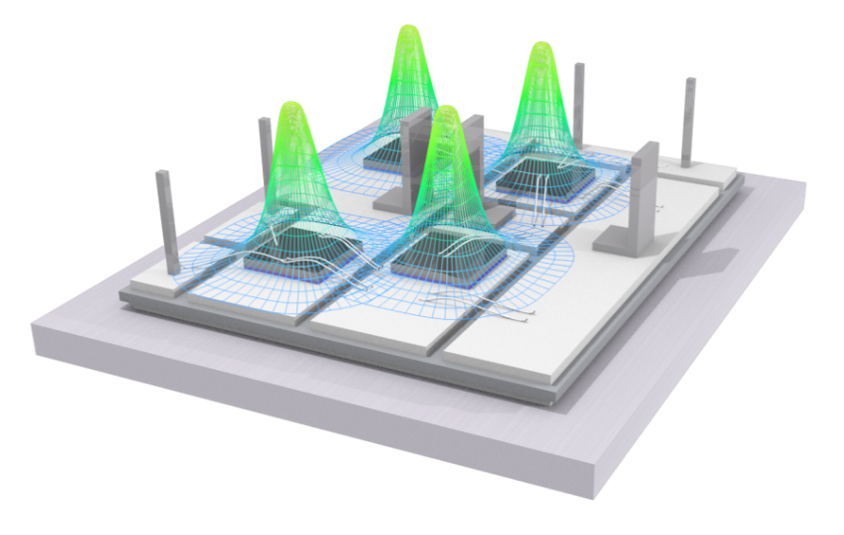
\includegraphics[width=\linewidth]{./figs/00_PS.png}
\end{figure}

\end{center}
\end{titlepage}

\tableofcontents
\pagebreak

\section{Introduction}
\label{sec-1}

\subsection{Executive Summary}
\label{sec-1-1}

PowerSynth currently performs multi-objective optimization to produce Pareto-front solutions to the proper placement of power semiconductor device die and the routing of metal traces on ceramic substrates. The tool accounts for temperature distributions and electrical parasitics as a function of the layout geometries that it considers. This tool has been hardware validated. Continued research on this project will further elaborate the capabilities by extending the work to greater fidelity in both the thermal and electrical domains.

Some of the major features of this tool include:
\begin{itemize}
\item Fast, accurate models for calculating electrical parasitics and thermal performance
\item Multi-objective optimization for layout synthesis
\item Able to synthesize and evaluate hundreds of layouts per minute
\item User can select multiple performance metrics for optimization
\item Built-in technology library including devices, substrates, attachment materials, bondwires, and more.
\item Manufacturer Design Kit for incorporating packaging house design rules and tolerances
\item Export designs to Ansys Q3D, FastHenry, or SolidWorks
\item Post-layout optimization for trace corner filleting
\item Easy to use GUI
\end{itemize}

\subsection{Organization}
\label{sec-1-2}

After a brief introduction to PowerSynth, this document walks the user through various features of PowerSynth by creating a new project in a step-by-step presentation. Following the walkthrough, some additional information on the Technology Library, Process Design Rules, and Layout Editor are presented.

\subsection{PowerSynth Overview}
\label{sec-1-3}

PowerSynth is an EDA tool with a friendly, graphical user interface for Multi-Chip Power Module (MCPM) layout synthesis. The tool is capable of importing a symbolic layout, which is an abstract layout representation of an MCPM, to automatically synthesize and generate multiple, real physical-layout solutions. This interface allows users to define technology libraries for power module materials, set up design constraints, and establish performance metrics for optimization. Additionally, export of optimal solutions is supported both graphically, on a 3D Solution Browser, and to modeling and analysis tools such as SolidWorks, Ansys Q3D, FastHenry, and Keysight EMPro. 

\begin{center}
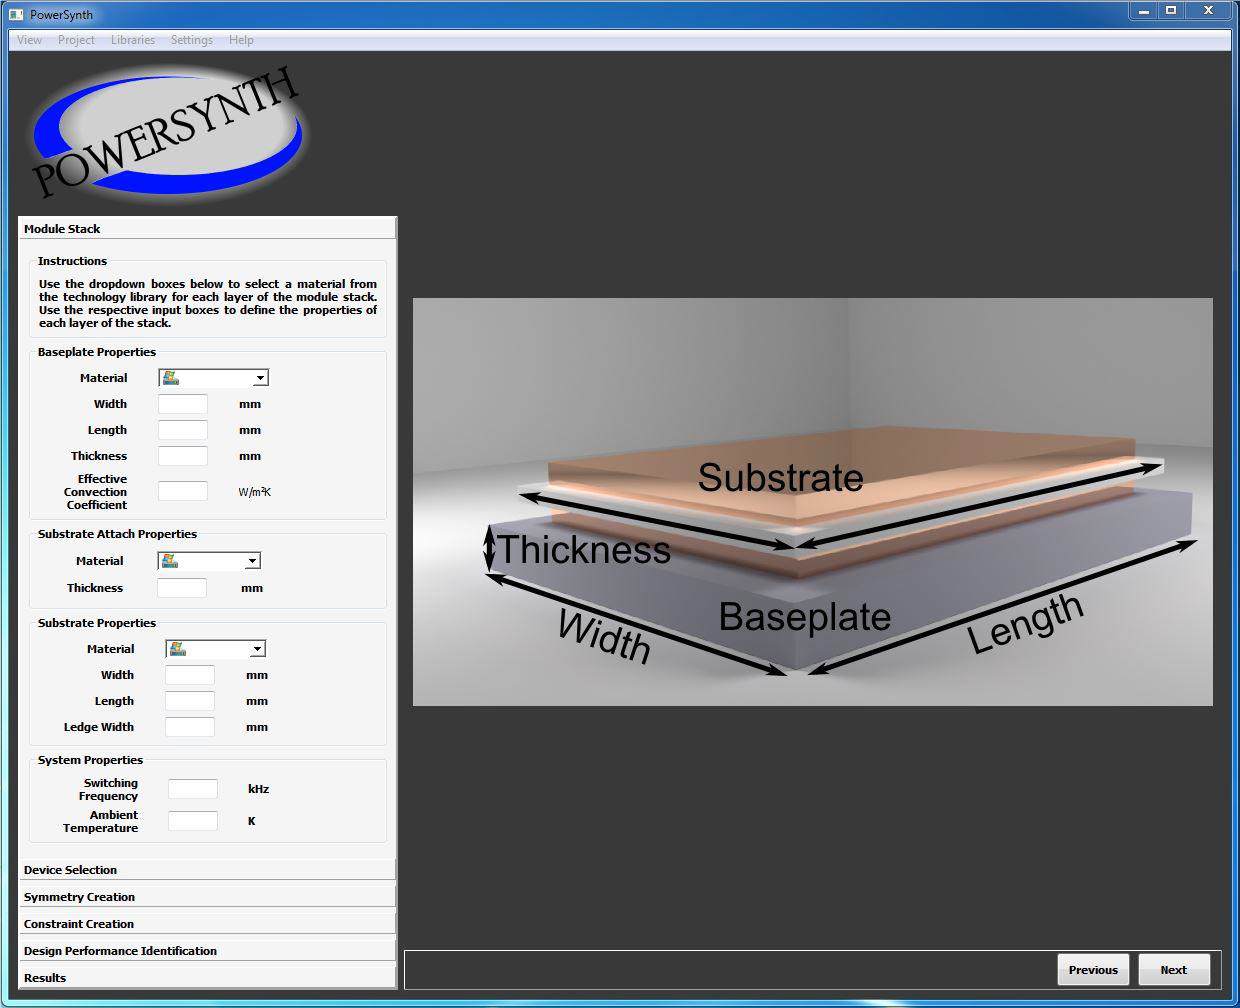
\includegraphics[width=14cm]{./figs/01_PSmain.png}
\end{center}

The layout optimization of PowerSynth is based on fast thermal and electrical parasitic models developed specifically for this tool. The thermal model uses spatial superposition of temperature distributions to determine the temperature of devices in a module. The temperature and heat flux distribution of each device is characterized from a single run of an automated FEM simulation. In this simulation, a single die is placed in the center of the module atop and un-patterned substrate. The top surface of this device is treated as the source of power dissipation and a heat transfer coefficient is applied to the backside of the module heat spreader.

A compact thermal model (CTM) is then constructed from the results of this simulation. Thermal resistance values for the CTM are found by placing the characterized temperature distribution for each device in superposition with neighboring ones. Heat flux distributions obtained in the characterization step are used to account for the interaction among devices given their positions on the current trace layout. Once the CTM is constructed, linear algebra techniques similar to those found in circuit analysis are used to predict the temperatures of each device. The model can predict changes in temperature over variations in trace layout and device positioning with a maximum error of less than 10\%. 

The electrical parasitics in a module are approximated by closed-form solutions to micro-strip transmission line models. Since all power modules share the same basic geometry, the micro-strip model provides a reasonably accurate representation of a power module’s trace parasitics. This is many times faster to execute when compared with finite element analysis. The electrical parasitic extraction works by breaking down a given layout into a lumped element network or graph with resistance and inductance values for each element or edge, approximated by micro-strip solutions. Capacitance from trace to baseplate (effective ground-plane) is evaluated at each lumped element node. These values can be used either directly in optimization or written into a netlist for simulation purposes. 

PowerSynth operates on an imported symbolic layout. This is a simple drawing of the topology of an initial module layout and is easy for a designer to create. A symbolic layout is comprised of three basic elements: lines, points, and rectangles. The line elements represent traces or bond wires. The point elements represent particular devices or leads, and the rectangle elements represent traces which span multiple traces vertically or horizontally in topological space. 
A designer chooses a set of performance metrics, in this case electrical or thermal, based on the symbolic layout. A multi-objective optimization problem is formulated based on the symbolic layout by allowing each layout line-element a variable width, which constitutes a set of design variables. The Non-dominated Sorting Genetic Algorithm II (NSGA-II) is used to perform the optimization procedure.

After the optimization routine is run, a particular layout can be selected from a set of trade-off solutions for the MCPM design, allowing the designer easy access to the entire, viable design space. This system also allows a designer to quickly test many different layout solutions while maintaining layout quality. The fast electrical and thermal models both predict temperature and parasitic values accurately with respect to FEM tools. 

\subsubsection{Constraint-Aware Layout Engine}
In this version, a constraint-aware layout engine has been integrated with PowerSynth. Now, there are two options for layout generation and optimization: 1) Using matrix-based layout engine (skip section 2.6), 2) Using constraint-aware layout engine (section 2.6). The significant improvements with the constraint-aware layout engine over the matrix-based one are: 
\begin{itemize}
    \item An interactive constraint input feature which is helpful for user to specify or modify design constraint values to have different layout structures.
    \item Four types of layout generation capability: minimum-sized layout, variable floorplan sized, fixed floorplan sized and fixed floorplan with fixed component locations, whereas the prvious one has only fixed floorplan sized layout generation capability.
    \item As the engine takes into account of all design constraints in the layout generation phase, it always generates 100\% valid solutions, whereas the matrix-based engine generates 20-30\% valid solutions due to design rule check(DRC)-failure.
    \item The matrix-based engine generates a non-smooth solution space and so gradient-based optimization algorithm cannot be used for optimization. But the updated layout engine can be used to test all different types of optimization algorithms. In this version two options are provided: NSGAII and non-guided randomization.
    \item Due to restricted input format (lines, points), the matrix-based engine is unable to process complex geometrical shapes in the layout. On the other hand, the updated layout engine treats each component as rectangle, so geometrical complexity is not a problem.
    \item The updated layout engine algorithms are more generic, scalable, and efficient than the matrix-based one. So, it can process broader range of layouts even considering heterogeneous components (e.g. gate drivers, EMI filters, sensors, etc.).
    \item As the updated layout engine is constraint-aware, different types of constraints can be declared : design constraints, reliability constraints, user-defined constraints. Generated solutions always satisfy all the given constraints.

\end{itemize}

In this beta-version, all of the features of the constraint-awrae layout engine are not integrated. Two layout engines are kept side-by-side, so that user can use both of the flows. The updated layout engine can take initial layout as a script describing all rectangle information that makes it more generic. However, in this version, the symbolic layout (lines, and points) format is considered as input format, which is automatically converted into rectangles in the constraint-aware layout engine for layout generation.

\textbf{Methodology}\\
From the user-defined initial input script, using corner stitch data structure (used in Magic VLSI tool), a collection of rectangular tiles are stored. Based on design constraints, constraint graphs (popular in VLSI floorplan compaction) are created from the corner-stitched plane. Two types of constraint graph are consdiered: horizontal constraint graph (HCG) and vertical constraint graph (VCG) for maintaining horizontal and vertical relationship among components. 

\begin{itemize}
\item \textbf{Constraints}:
Three types of design constraints are considered.
\begin{enumerate}
    \item \textbf{Dimension Constraints}: Here, minimum width along x-axis (Min Width), minimum width along y-axis and minimum enclosure are specified for each type of component. Currently, only trace, mos, diodes, and leads are considered. 
    \item \textbf{Spacing Constraints}: In this table, minimum spacing values between every pair of components are declared. 
    \item \textbf{Enclosure Constraints}: When a component is placed on top of another component, there may be some minimum enclosure value. So, this table has all possible minimum enclosure values.
\end{enumerate}
\item \textbf{Operating Modes}

Based on the evaluation of the constraint graphs, there are four modes of operation (shown in Table ~\ref{T.operating modes}).

\begin{table}[H]
\caption{SUMMARY OF OPERATING MODES}
\label{T.operating modes}
\begin{tabular}{|c|c|c|}
\hline
\textbf{Mode} & \textbf{Purpose} & \textbf{Evaluation Methodology} \\ \hline
0 & Minimum sized layout & Minimum constraint values \\ \hline
1 & Variable floor-plan layouts & \begin{tabular}[c]{@{}c@{}}All weights are randomized with minimum constraints.\\  No maximum constraints\end{tabular} \\ \hline
2 & Fixed floor-plan layouts & \multirow{\begin{tabular}[c]{@{}c@{}}All weights are randomized with minimum constraints. \\ Some have maximum constraints\end{tabular}} \\ \cline{1-2}
3 & \begin{tabular}[c]{@{}c@{}}Fixed floor-plan with \\ fixed component locations\end{tabular} &  \\ \hline
\end{tabular}
\end{table}
\begin{itemize}
    \item \textbf{Minimum Size Layout}: This layout is generated using all minimum constraint values. So, this layout reflects maximum possible power density for a layout. As this is the minimum sized solution, it is electrically optimized but thermal performance is so poor.
    \item \textbf{Variable Size Layout}: If this mode is selected, all constraint values are randomized and new layout solution is generated. User can generate arbitrary number of valid layout solutions with different floorplan size.
    \item \textbf{Fixed Size Layout}:  All edge weights are randomized within given area to generate arbitrary number of solutions. As floorplan size is always fixed there is less variation in this mode than the previous one.
    \item \textbf{Fixed Size with Fixed Locations}: This mode is useful for packaging purpose. If any component is to be always fixed at certain location throughout all solutions, this mode should be used. User can choose any absolute location at which any component needs to be fixed. In this mode, user can also generate arbitrary number of layouts.
\end{itemize}
 All algorithms can be found in "WIPDA\_2018.pdf" in the Publication folder.
\end{itemize}

\pagebreak

\section{Using PowerSynth}
\label{sec-2}

\subsection{Installing PowerSynth}
\label{sec-2-1}

\begin{enumerate}
\item Run the PowerSynth install wizard
\item Run PowerSynth.exe
\end{enumerate}
\par
\textbf{Note:} It is STRONGLY RECOMMENDED that you install PowerSynth in the C drive (the default installation directory) and NOT in Program Files. Installing PowerSynth in Program Files can result in various issues relating to administrator permissions.
\par
\textbf{Note:} This version of PowerSynth is meant to work with the tool ParaPower by the Army Research Laboratory. As such, \textbf{MATLAB 2020b} must be installed before PowerSynth is run. After installation, make sure that the the variable \textbf{MATLAB\_BIN\_DIR} in the file \emph{C:/PowerSynth/MATLAB/settings.txt} points to the appropriate path in your MATLAB installation folder, e.g. \par \emph{C:/Program Files/MATLAB/R2020b/bin/win64}.

\subsection{Creating a New Project in PowerSynth}
\label{sec-2-2}

\subsubsection{User Interface}
\label{sec-2-2-1}

\begin{wrapfigure}{r}
\centering
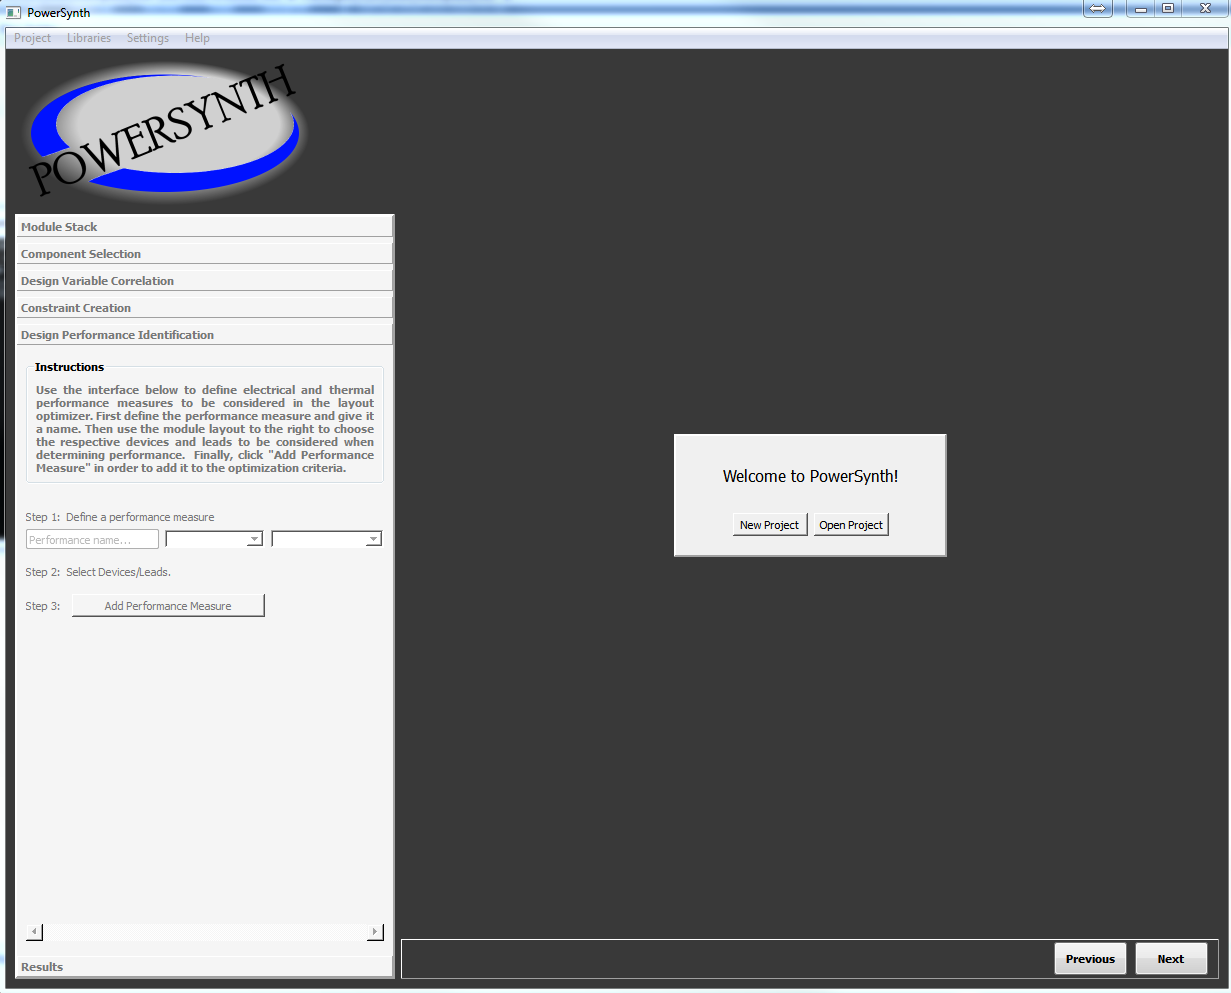
\includegraphics[width=10cm]{./figs/02_NewProj.png}
\end{wrapfigure}

The welcome screen is shown on the right. The navigation pane on the left is used to develop a project once a new project is created or an existing project is opened. Before we click “New Project”, we need to define the layout template that will be imported.

\subsubsection{Symbolic Layout File}
\label{sec-2-2-2}

A symbolic layout is a simple stick diagram used to represent a simple power module’s abstract layout. In the previous version, PowerSynth relies on InkScape to create a SVG file. This SVG file represents a stick diagram which is then imported into PowerSynth for a new project. In this version, SVG feature has been removed due to some unstable functionalities. Instead, the user can provide a script (text file) to define the stick diagram.  Each point on this stick diagram represents either a device or a lead, while each line represents a trace. Bondwires information will need to be provided later in the setup (see Assigning Virtual Wires Connections). This script must be created before creating a new project in PowerSynth.  Open a text file and define the layout template using lines and points with the syntax as shown below. Lines denote traces, while points denote devices and leads. Below is a sample layout script. It is of the format: 

\textbf{Name Type (x1,y1) (x2,y2)}

Note: The element name (first column) must be four characters long.
For a point, (x1, y1) is the coordinate of the point.
For a line, (x1, y1) is one of the end points. (x2, y2) is the other endpoint. 
Save this file in either .psc or .txt format.

\pagebreak

The example script for the symbolic layout is shown below:
\begin{wrapfigure}{r}{0.8\textwidth}
\centering
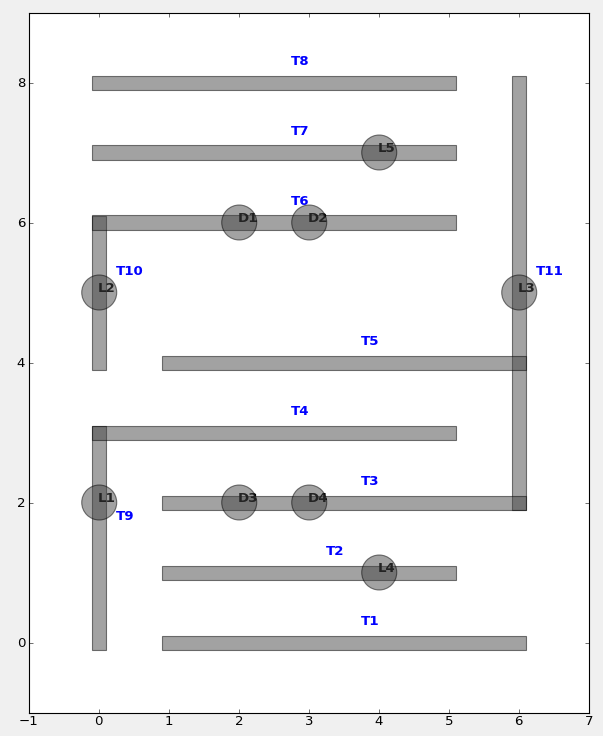
\includegraphics[width=0.4\textwidth]{./figs/03_SymLayout.png}
\end{wrapfigure}


\texttt{T1 l (1,0) (6,0)}

\texttt{T2 l (1,1) (5,1)}

\texttt{T3 l (1,2) (6,2)}

\texttt{T4 l (0,3) (5,3)}

\texttt{T5 l (1,4) (6,4)}

\texttt{T6 l (0,6) (5,6)}

\texttt{T7 l (0,7) (5,7)}

\texttt{T8 l (0,8) (5,8)}

\texttt{T9 l (0,0) (0,3)}

\texttt{T10 l (0,4) (0,6)}

\texttt{T11 l (6,2) (6,8)}

\texttt{D3 p (2,2)}

\texttt{D4 p (3,2)}

\texttt{D1 p (2,6)}

\texttt{D2 p (3,6)}

\texttt{L1 p (0,2)}

\texttt{L2 p (0,5)}

\texttt{L3 p (6,5)}

\texttt{L4 p (4,1)}

\texttt{L5 p (4,7)}



\bigskip
\bigskip
\bigskip

Note that these coordinate values are not real coordinates and thus have no dimensional units. These coordinates are used to find the relative position of each line and point to each other. Once this file is imported to the software, an automatic normalization algorithm will run to count the number of rows and columns. These coordinates are then normalized between zero and the maximum number of rows/columns. The corresponding symbolic layout for the abovementioned script is represented on the left. Once the project is loaded, the layout can still be modified using the Layout editor under \textbf{Project -> Open Layout Editor}

\pagebreak

\subsubsection{Create a New Project}
\label{sec-2-2-3}

\begin{wrapfigure}{r}
\centering
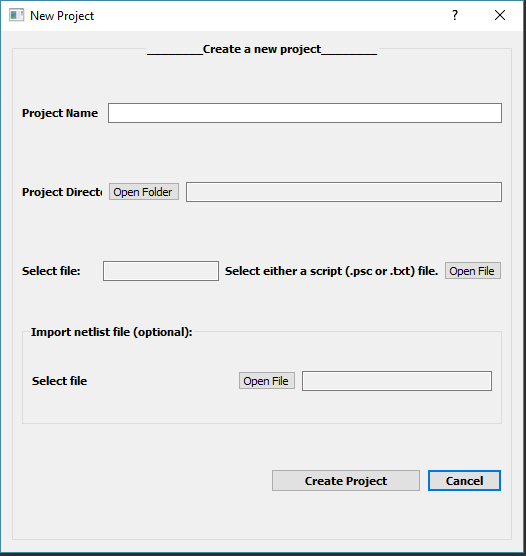
\includegraphics[width=0.5\textwidth]{./figs/04_NewProj.png}
\end{wrapfigure}

Selecting the “New Project” button on the welcome window brings up the dialog for a new project as shown on the right. First, give the project a name. Then, select the folder where it will be saved. Import the symbolic layout file as shown above using “select file”. Select the directory where you saved the text file. Finally, click “Create Project”. 

\emph{Optional:}
The user can also specify a netlist file that have same circuit topology with the symbolic layout. 
This can be later used to map the net names with the symbolic layout object. A sample netlist format for a 4 switches half bridge is shown below:

\begin{verbatim}
*Sample Netlist file:*
M1 DC_plus G_High Out Out NMOS
M2 DC_plus G_High Out Out NMOS
M3 Out G_Low DC_neg DC_neg NMOS
M4 Out G_Low DC_neg DC_neg NMOS
.model NMOS NMOS
.model PMOS PMOS
.end
\end{verbatim}

\subsection{Defining the Module and Components}
\label{sec-2-3}
\subsubsection{Module Stack}
\label{sec-2-3-1}

The module stack tab on the left allows the user to input module stack information for the design. This includes dimension and material information of the substrate, substrate attach and baseplate. Operating conditions such as ambient temperature, effective convection coefficient of baseplate and switching frequency are also required for thermal and electrical evaluations.  The user can update the tech files (\textbf{.p) using * Libraries->Tech lib}.

\begin{center}
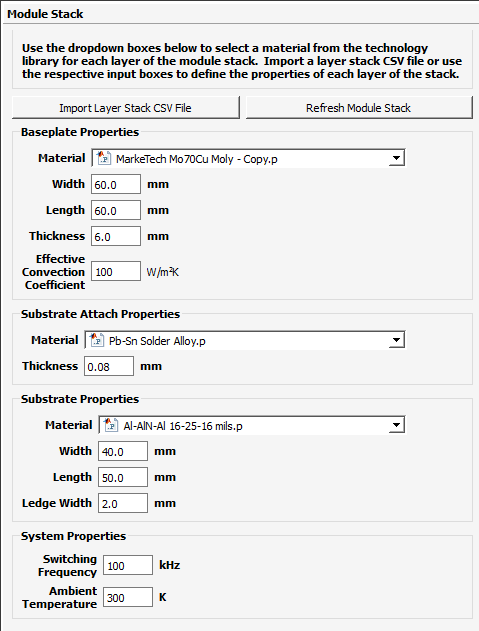
\includegraphics[width=8cm]{./figs/05_LayerStack.png}
\end{center}

Another way to import this module stack is through a csv layer stack file. The description for this file is explained in the next section.

\subsubsection{Layer Stack File}
\label{sec-2-3-2}

\begin{longtable}{lrlrrrrl}
\textbf{Abbrev} & \textbf{LayerID} & \textbf{Name} & \textbf{Layer} & \textbf{Width} & \textbf{Length} & \textbf{Thickness} & \textbf{Material}\\
 &  &  & \textbf{Position} &  &  &  & \\
\hline
\endhead
\hline\multicolumn{8}{r}{Continued on next page} \\
\endfoot
\endlastfoot
B: & 1 & B1 & 1 & 45 & 45 & 6 & copper\\
SA: & 2 & SA1 & 2 & 40 & 40 & 0.08 & solder\\
M: & 3 & M1 & 3 & 38 & 38 & 0.41 & copper\\
D: & 4 & D1 & 4 & 40 & 40 & 0.64 & Al$_{\text{N}}$\\
I: & 5 & I1 & 5 & 28 & 28 & 0.41 & copper\\
C: & 5 & C1 & 6 & 2.5 & 4 & 0.2 & SiC\\
\end{longtable}

The Table above shows the module stack structure. The user can specified this in an excel (.csv) and load it using the \textbf{Import Layer Stack File} button in the UI.

Some Abbreviation: B: Baseplate, SA: Substrate Attach, M: Metal, D: Dielectric, I: Interconnect (Metal), C: Component (this is optional for this version).

Below shows the UI after successfully importing the layer stack. To go back to the normal mode, press the \textbf{Refresh Module Stack} button.

\begin{center}
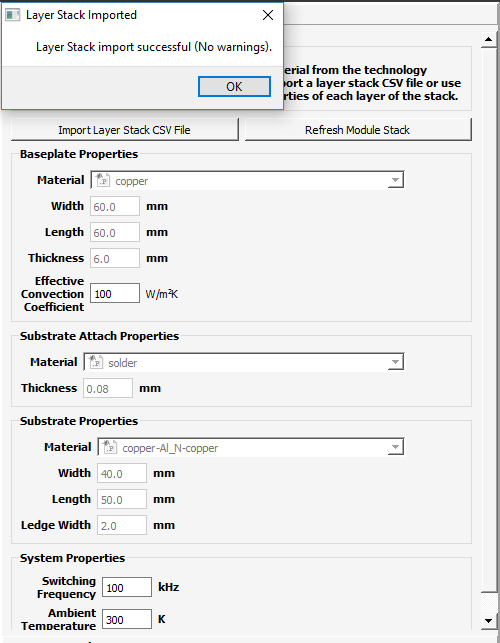
\includegraphics[width=8cm]{./figs/06_LayerStack2.png}
\end{center}

\subsubsection{Component Selection}
\label{sec-2-3-3}

The symbolic layout is shown on the right side of the interface. This allows users to insert component technology files. These files contain information about the bondwires, leads, and devices the user wishes to include. Notice that the names from the layout script for each traces and Devices are shown on the right-hand side. (Symbolic Layout)

\begin{center}
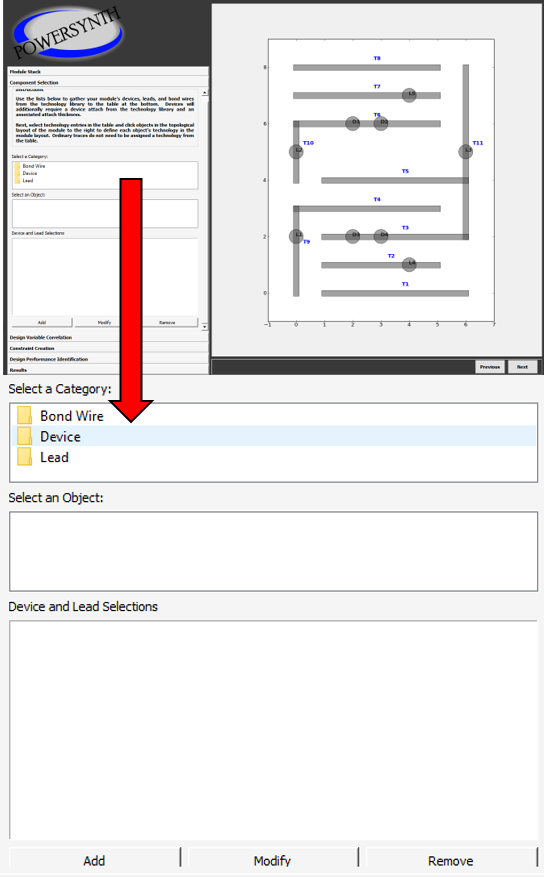
\includegraphics[width=12cm]{./figs/07_Components.png}
\end{center}

The user can assign devices and leads to the circles on the symbolic layout. The unassigned lines will represent copper or aluminum traces (depending on substrate selection). Wires bond will be treated as virtual connections. However, it is recommended to finish the devices and leads selection first before assigning virtual wire bonds to ensure correct connection.

\pagebreak

\subsubsection{Device and Lead Selection}
\label{sec-2-3-4}

\begin{wrapfigure}{r}{0.6\textwidth}
\centering
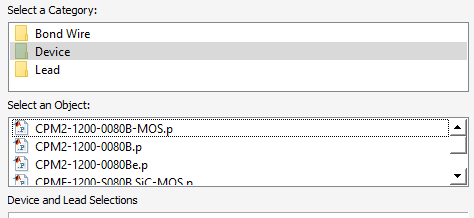
\includegraphics[width=0.6\textwidth]{./figs/08_Components2.png}
\end{wrapfigure}

Click on “Device” or “Lead” from the Category list, a list of objects under object selection will be listed out. This can be specified using the TechLib (See Technology Editor section)

Once an object is selected, press the “Add” button. In case of device, this will pull up a dialog on the right to define the solder type (tech lib), solder thickness and average power of the device. This information will be used for thermal optimization. Click Done to apply this for the device. This will update the device and lead selection table. 
The user can do the same for the lead selection to fill the Device and Lead Selection table on the right.

\begin{center}
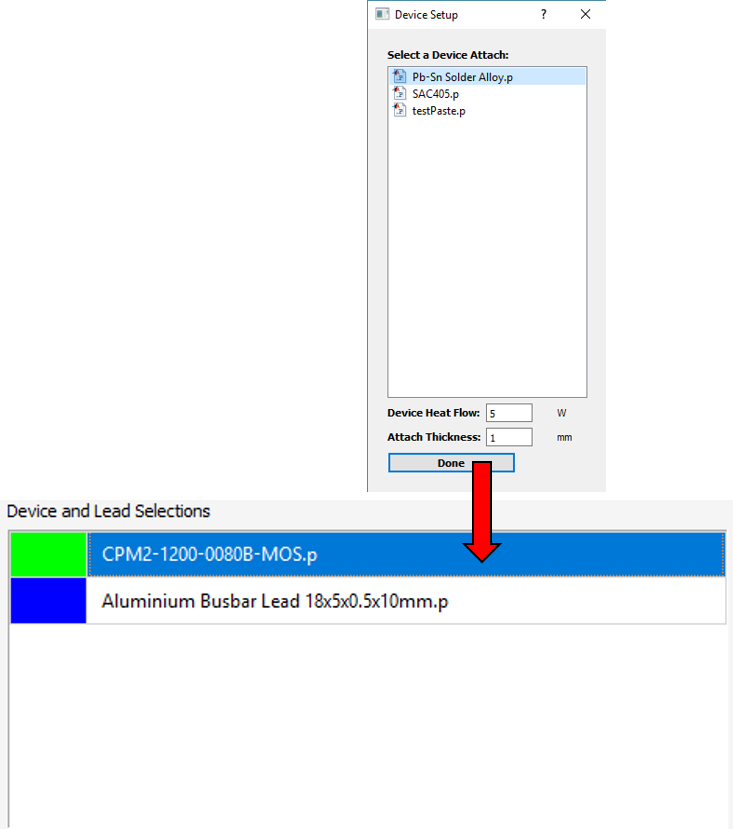
\includegraphics[width=10cm]{./figs/09_DeviceSetup.png}
\end{center}

\pagebreak

\subsubsection{Assigning Devices and Leads}
\label{sec-2-3-5}

\begin{wrapfigure}{r}{0.6\textwidth}
\centering
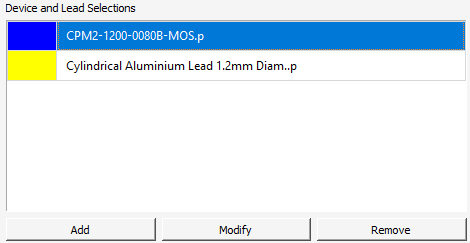
\includegraphics[width=0.6\textwidth]{./figs/10_DeviceLead.png}
\end{wrapfigure}

First, select a device or lead object from the table.

Assigining these selections on the Symbolic Layout by clicking on the circles. To deselect, click on the selected circle one more time. The circles will be colored based on the random generated color on the Device-Lead Table.
In case the user imported a netlist (Create new project section), a small dialog will be trigged to select the corresponded net name.

\begin{center}
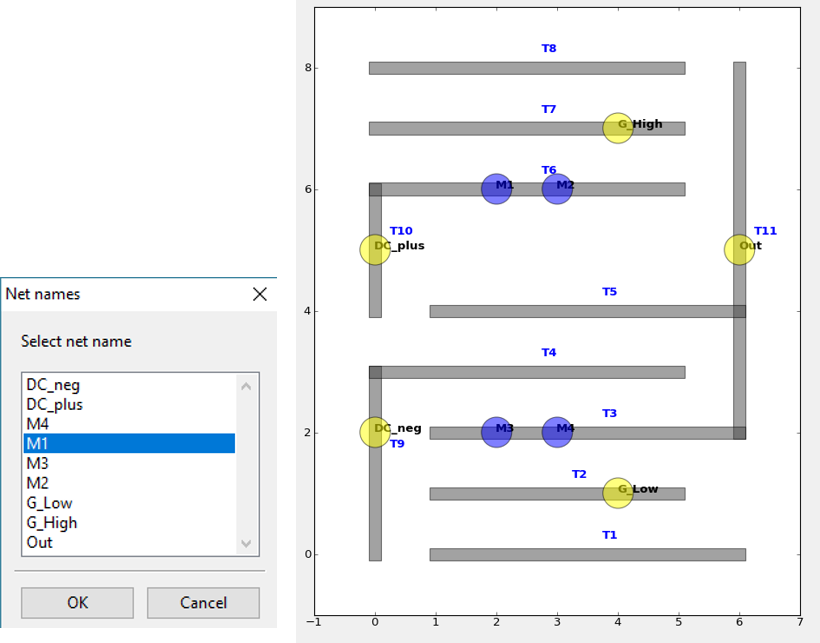
\includegraphics[width=10cm]{./figs/11_NetNames.png}
\end{center}

\pagebreak

\subsubsection{Assigning Virtual Wire Connections}
\label{sec-2-3-6}
\begin{wrapfigure}{r}
\centering
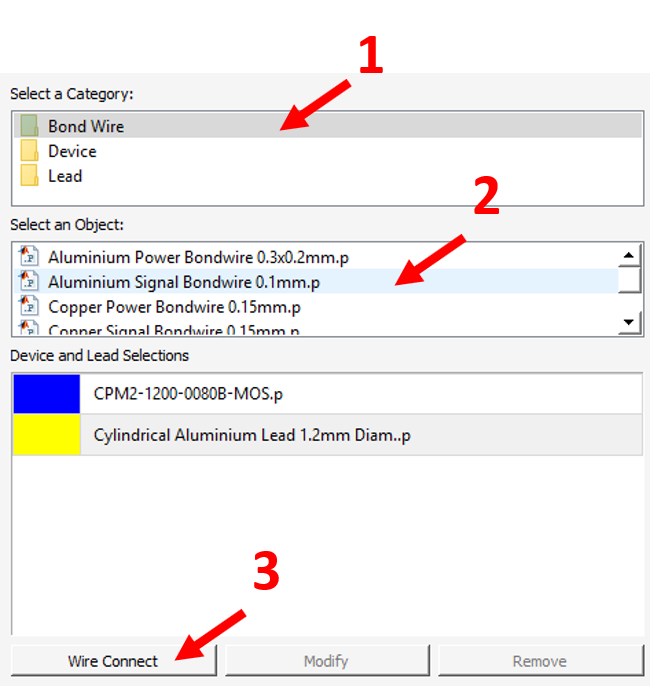
\includegraphics[width=0.5\textwidth]{./figs/12_BW.png}
\end{wrapfigure}

Once all of the devices and leads are setup like above, the next step is to setup the virtual wires connections. To do this, first click on “Bond Wire” from the categories selection list. Then, select a bondwire object. The “Add” button will change its text to “Wire Connect” as seen on the right:

A bond wire Setup dialog will open as seen on the right. The symbolic layout is now in wire selection mode. The user will need to select 2 traces or a trace and a device (device to device bondwire is not supported yet) for wire connections.
For a MOSFET, it is required to have signal and power wires for signal and source sides.
To select 2 objects, simply click on the symbolic layout again. The selected object will be hatched as shown below.

The \textbf{Add} buton on the dialog will be enabled if 2 objects are selected (click again if you want to deselect an object). Click this to add the wire connection to the table. Doing so, we can have a complete table (on the left). Close the dialog, the table can be saved and edited any time.

\bigskip


\begin{center}
\begin{tabular}{p{0.4\textwidth}p{0.4\textwidth}}
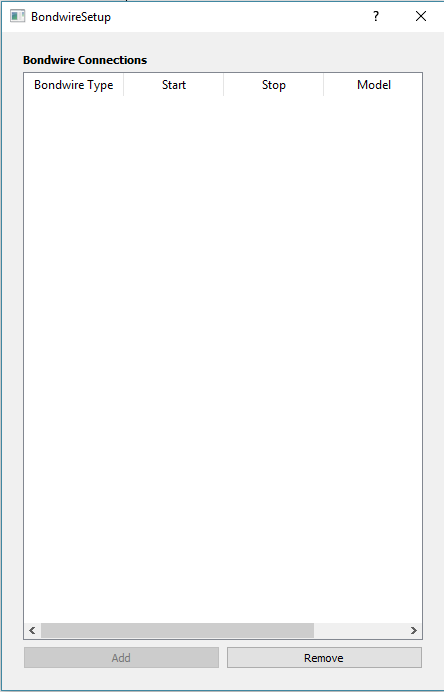
\includegraphics[width=.9\linewidth]{./figs/13_BW2.png} & 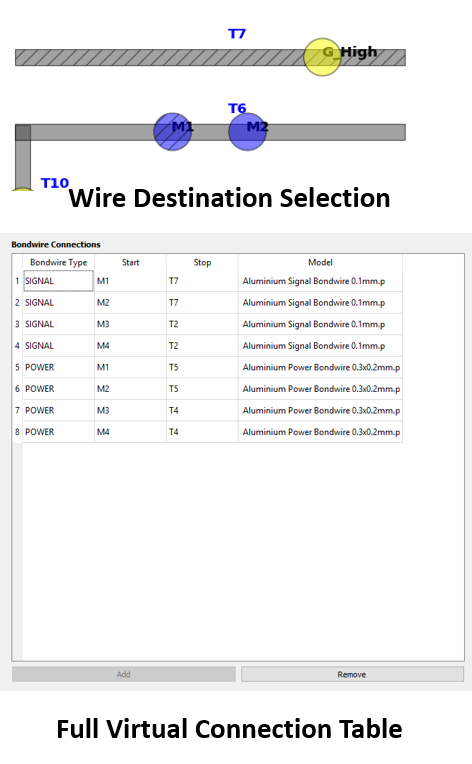
\includegraphics[width=.9\linewidth]{./figs/14_Vconn.png}\\
\end{tabular}
\end{center}


\pagebreak

\subsection{Defining Correlations and Constraints}
\label{sec-2-4}
\subsubsection{Design Variable Correlation}
\label{sec-2-4-1}

If symmetrical traces or device positions are desired in the design, correlation between devices or traces can be assigned.  This will ensure that selected traces will have the same width (length) or that selected devices will have same position. Click “Add New Correlation” and a new row will appear in the table. Click on a row then click on traces or devices to specify a correlation.

\begin{center}
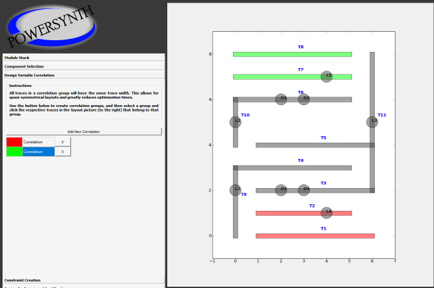
\includegraphics[width=0.7\textwidth]{./figs/15_Corr.png}
\end{center}

\subsubsection{Constraint Creation}
\label{sec-2-4-2}

Here, the user can click on each line (trace) to specify a min and max or fixed width for a trace. If there are symmetry constraints, these will be applied to all symmetric traces. 

\begin{center}
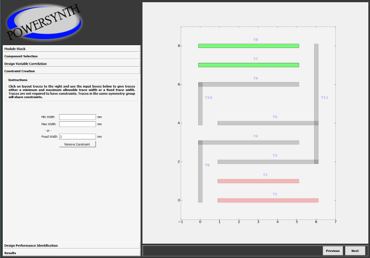
\includegraphics[width=0.7\textwidth]{./figs/16_Const.png}
\end{center}

\pagebreak

\subsection{Design Performance Identification}
\label{sec-2-5}

In this step, the user can choose the performance metrics that are to be optimized.  The next two sections below show the process for assigning performance metrics. Once the performance metrics are selected, the user can go to the next tab to run the design optimization. Currently, PowerSynth supports thermal and electrical measurement of a power module.

\subsubsection{Thermal Measurement}
\label{sec-2-5-1}

On the navigation tool, a user can define a performance measure. There are 2 available thermal models in PowerSynth: Rectangle Flux (analytical) and Fast Thermal (Characterized by FEM simulation). In case of thermal measurement, follow the steps below:

\begin{center}
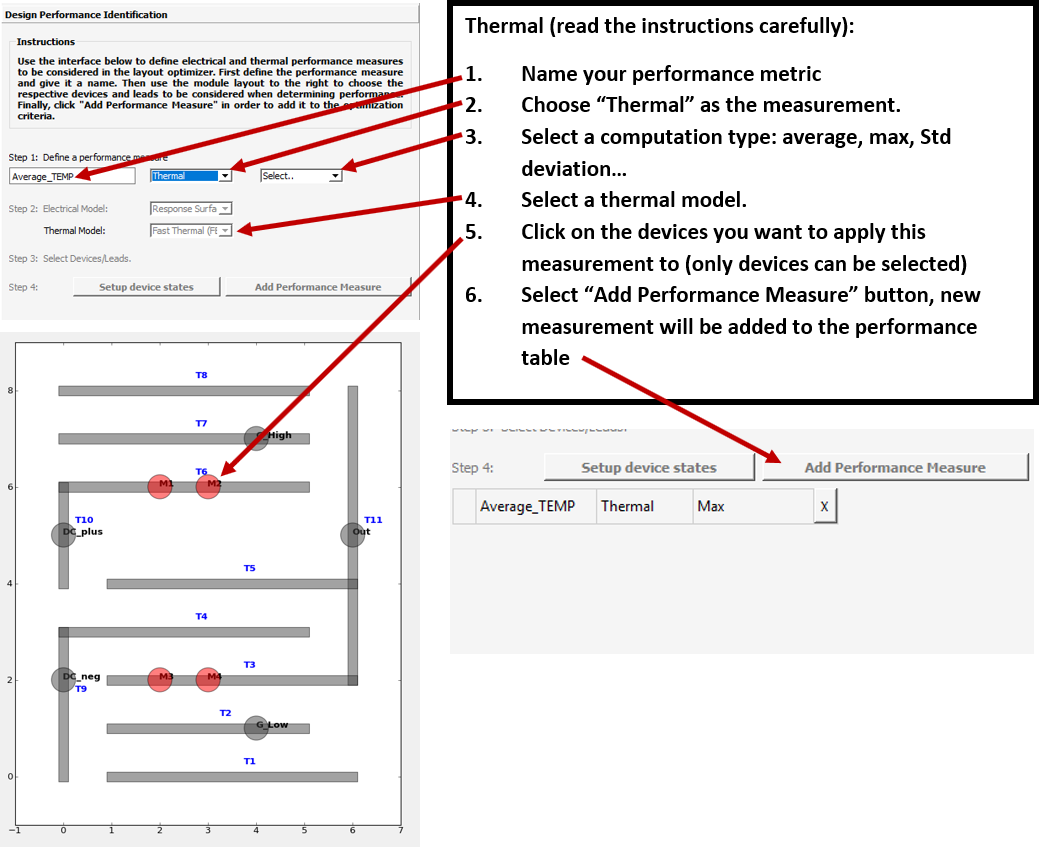
\includegraphics[width=0.7\textwidth]{./figs/17_thermal.png}
\end{center}

\subsubsection{ARL ParaPower Thermal Analysis}
\label{parapower}

As part of a collaborative project with the US Army Research Lab (ARL), an API has been developed to utilize their tool, \href{https://github.com/USArmyResearchLab/ParaPower}{ParaPower}, within the PowerSynth optimization routine. ParaPower provides quick steady-state and transient thermo-mechanical analysis capabilities that can be applied toward the electro-thermo-mechanical co-design of power modules. A brief overview of how the ParaPower API used by PowerSynth is shown below. Additionally, more information regarding this work can be found in ECCE article mentioned in \ref{sec-4}.

\begin{center}
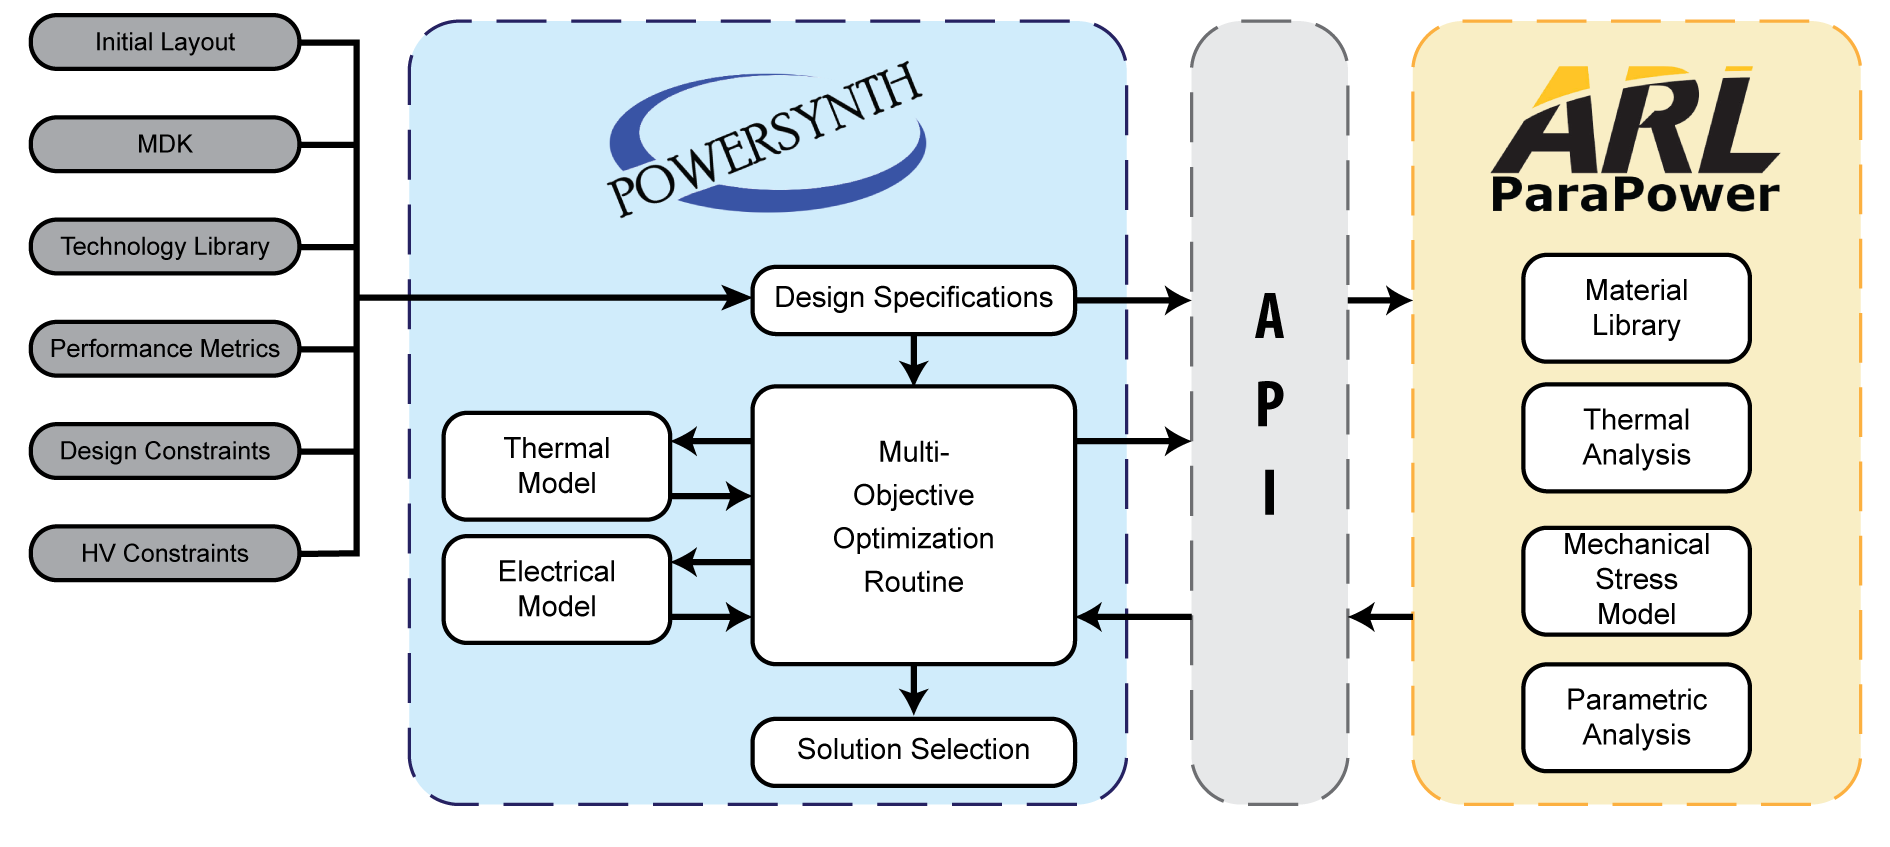
\includegraphics[width=0.8\textwidth]{./figs/ParaPower/CODESIGN_r1-01.png}
\end{center}

While access to the full analysis capabilities of ParaPower are available through the developer version of this API, for this release of PowerSynth (v1.4) only steady-state thermal analysis is supported. One other caveat is that this is meant to work with the legacy “symbolic layout” power module representation used in PowerSynth and not the newer, layer-stack representation.

To use ParaPower steady-state thermal analysis as a design performance criterion, similar steps are performed as in section \ref{sec-2-5-1}. The main difference being that when choosing the thermal model, the “ParaPower Thermal Model” option should be selected as shown below:

\begin{center}
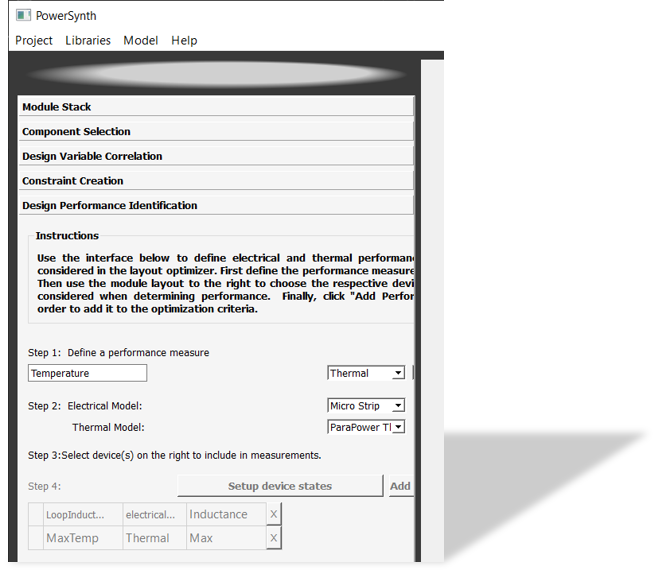
\includegraphics[width=0.7\textwidth]{./figs/ParaPower/ParaPowerDesignPerformance_Thermal.png}
\end{center}

ParaPower offers additional boundary condition settings beyond what this release of PowerSynth considers using the built-in thermal models. The built-in PowerSynth modules only consider temperature and heat transfer from the module backside. Whereas, with ParaPower, these conditions may be specified for all six faces of a rectangular prism enclosing the power module design. 

ParaPower analysis boundary conditions and solver settings can be accessed at any point prior to optimization in PowerSynth by choosing “ParaPower Setup” from the “Model” drop-down on the main menu as shown below. Values are automatically populated from the information provided in the “Module Stack” settings pane. Note that these are automatically chosen to mimic the boundary conditions of the other PowerSynth thermal models. If boundary temperature and heat transfer values for any of the other five faces are to be specified, they can be entered manually, here. Once all settings are entered, press "Save" to write the changes prior to optimization.

\begin{center}
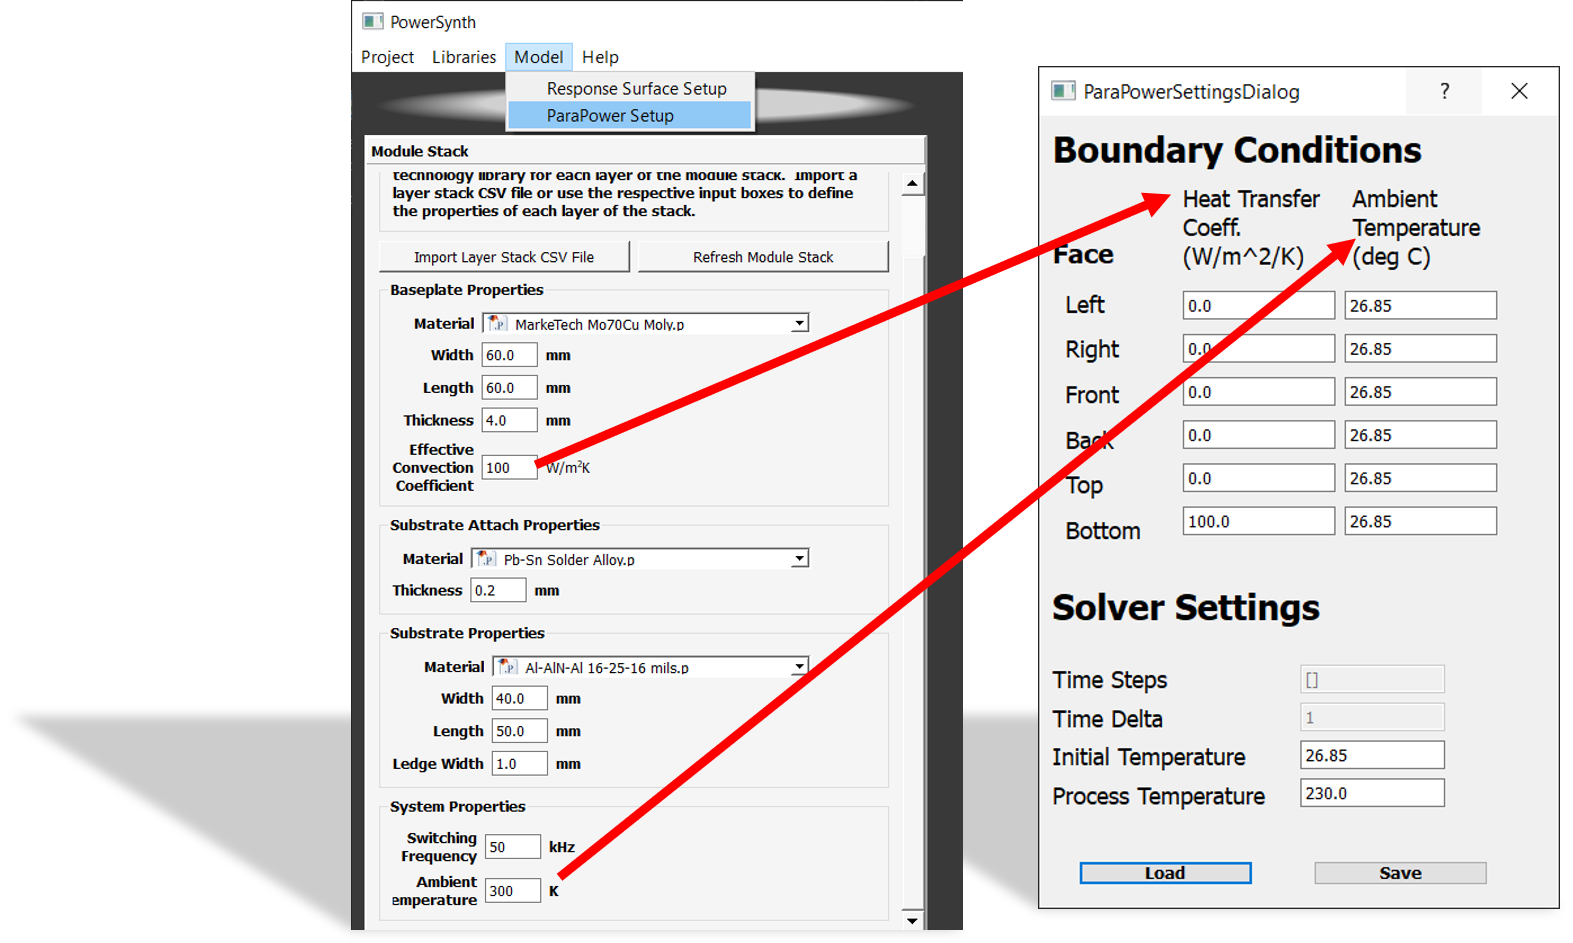
\includegraphics[width=0.8\textwidth]{./figs/ParaPower/ParaPowerSettings.png}
\end{center}

After ParaPower setup has been completed, along with choosing the ParaPower Thermal design performance criterion, PowerSynth optimization can be executed as normal  with the maximum temperature results being added to the solution Pareto frontier.


\pagebreak

\subsubsection{Electrical Measurement}
\label{sec-2-5-2}

Parasitic capacitance, resistance, and inductance can each be specified as design performance metrics to be optimized. The next few sections will detail the steps necessary to define them and build response surface models for quick evaluation.

\subsubsection{Inductance and Resistance Measurement}
\label{sec-2-5-3}

\begin{center}
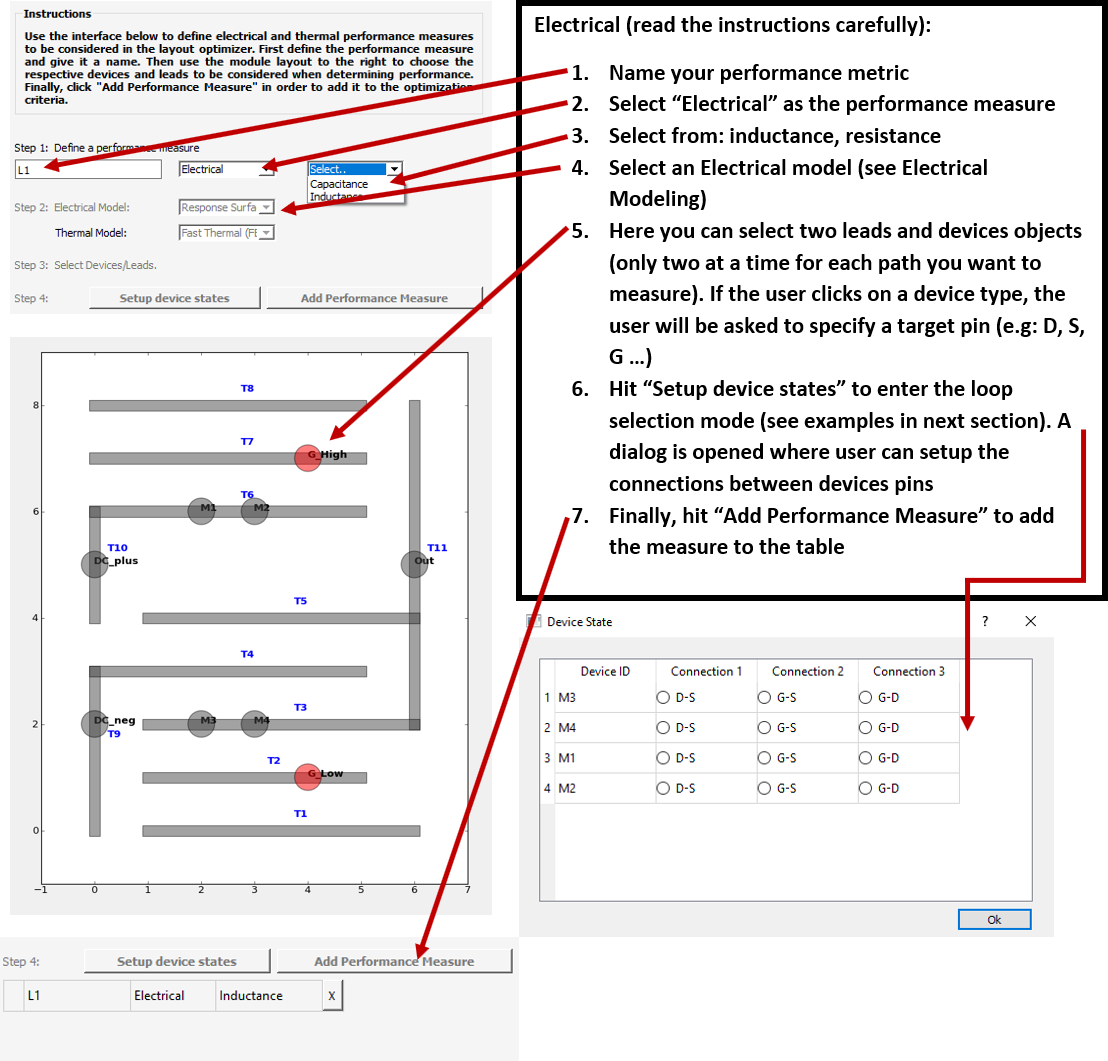
\includegraphics[width=0.7\textwidth]{./figs/18_electrical.png}
\end{center}

\pagebreak

\subsubsection{Device Connection Setup (Example)}
\label{sec-2-5-4}

Although on the symbolic layout devices are represent as nodes (circles), in a real power module layout, these devices have real dimension and several connection pads. By default, there are no connections between these pads (usually a capacitance if this is a MOSFET). To give the user the flexibility to select different loops, the setup device connection feature is used to select virtual connections between any two pins of a given devices. For example, from the same electrical measurement above, we can setup 2 different loops.

\textbf{Loop 1:}

Setup the device connections as follows:

\begin{center}
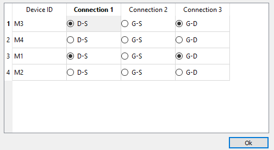
\includegraphics[width=8cm]{./figs/19_dconn.png}
\end{center}

We now have the following loop:

\begin{center}
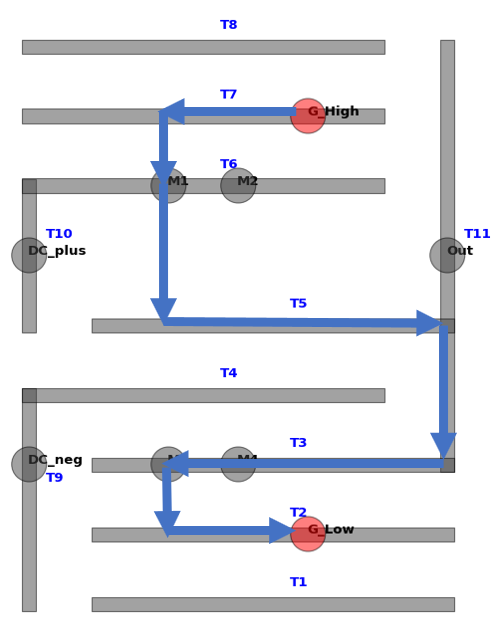
\includegraphics[width=8cm]{./figs/20_Vloop.png}
\end{center}

Name this loop as \texttt{L1} and add this to the table.

\subsubsection{Electrical Modeling}
\label{sec-2-5-5}

Under the electrical model selection on the UI, the analytical microstrip option can provide quick estimation of the inductance and resistance results. However, there are several drawbacks for this model such as not-frequency dependent, and usually less accurate for big traces. To overcome this problem, a response surface option is also provided. This model can be characterized using FastHenry or Q3D. To open the model creator, the user can go to: \textbf{Model -> Response Surface Setup}. A dialog as seen below is opened:

\begin{center}
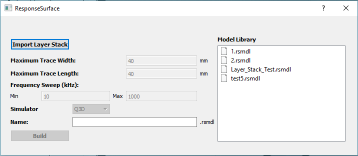
\includegraphics[width=10cm]{./figs/21_Emodel.png}
\end{center}

\begin{enumerate}
\item \textbf{Import Layer Stack:} this is explained in the Module Stack section below, this defines the baseplate and substrate dimensions. Different baseplate structures can affect the inductance calculation.

\item \textbf{Defining Maximum Trace Width and Length:} minimum trace width and length are based on minimum trace width in the Design Rule Check from PowerSynth (See Process Design Rules Editor). Define the maximum length and width here to characterize the model

\item \textbf{Defining Frequency sweep:} Specify the minimum and maximum frequency in KHz. The maximum frequency will define the minimum mesh in the characterization.

\item \textbf{Simulator:} 2 simulators are available now. These include ANSYS Q3D and FastHenry, the default ANSYS directory is: \texttt{C:\textbackslash{}Program Files\textbackslash{}AnsysEM\textbackslash{}AnsysEM18.2} (Versions up to 18.2 are supported). Another option is FastHenry (recommended), this is an open source parasitic extraction tool from MIT. The exe file for FastHenry is included in the package.

\item \textbf{Model name:}  Model name can be specified by user. This will be later added to the model library on the right.

\item \textbf{Build:} Once everything is setup, hit “build” button. Depending on the Simulator choice, and maximum frequency, the model will be built within 15\textasciitilde{}30 minutes.
\end{enumerate}

\begin{center}
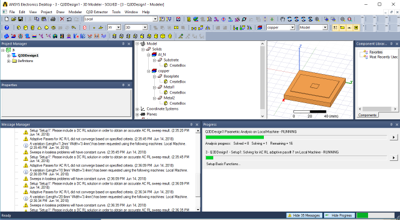
\includegraphics[width=10cm]{./figs/22_RS1.png}
\end{center}

The simulation is automatically run in Q3D to characterize the model. If FastHenry simulation is selected this will be run in the back-end (Command Prompt) of the tool.

\begin{center}
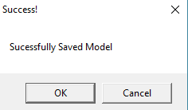
\includegraphics[width=4cm]{./figs/23_RS2.png}
\end{center}

A dialog shows up when the simulations are done. Click Ok to go back to PowerSynth UI.

If the model is selected in the design performance selection, a dialog will be opened. The user can select the models from the list:

\begin{center}
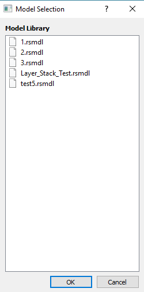
\includegraphics[width=4cm]{./figs/24_RS3.png}
\end{center}

\pagebreak

\subsubsection{Capacitance}
\label{sec-2-5-6}

\begin{center}
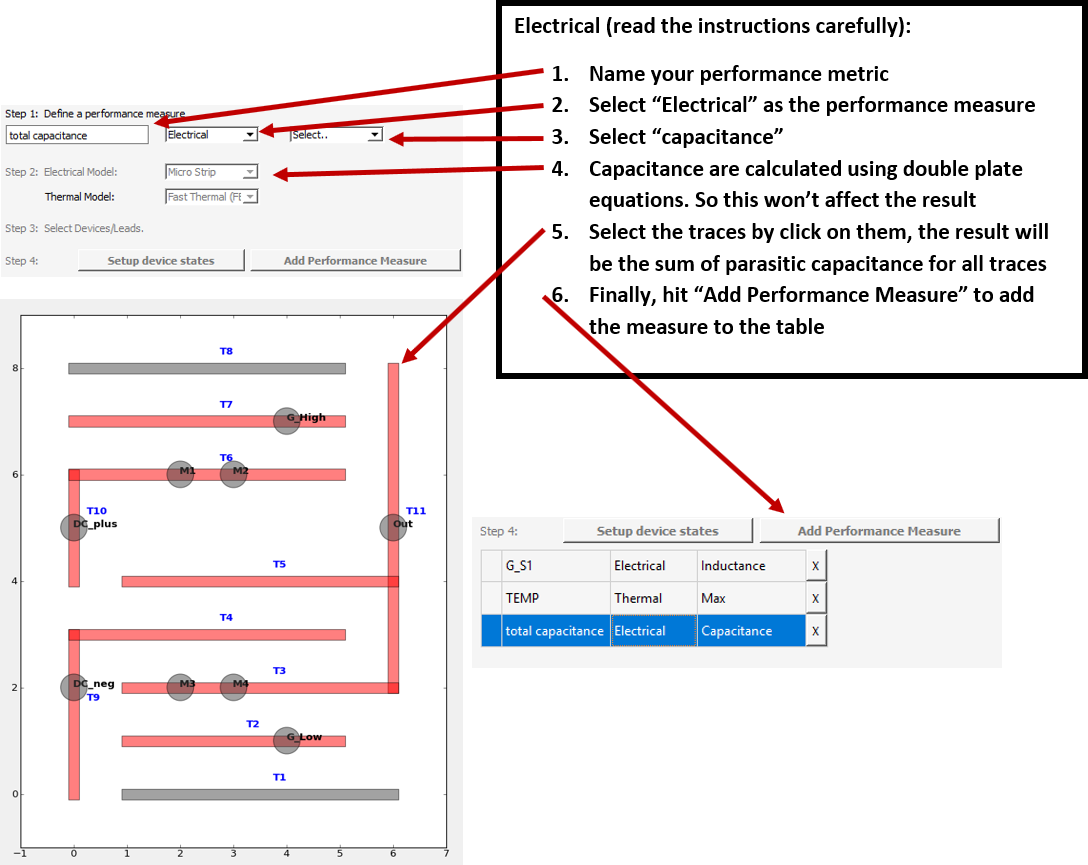
\includegraphics[width=0.7\textwidth]{./figs/25_Capacitance.png}
\end{center}

\pagebreak

\subsection{Constraint-Aware Layout Engine (Beta-Version)}
\label{sec-2-6}
To use this layout engine, the user must follow the steps up to \ref{sec-2-3-6}. Then constraint-aware layout engine button will be enabled. Upon clicking on the button (marked with an arrow in Fig.~\ref{start_w}) named \textbf{“Constraint-Aware Layout Engine”} the updated layout engine dialog will appear (shown in Fig.~\ref{new_dialog}).
\begin{figure}[h]
\centering

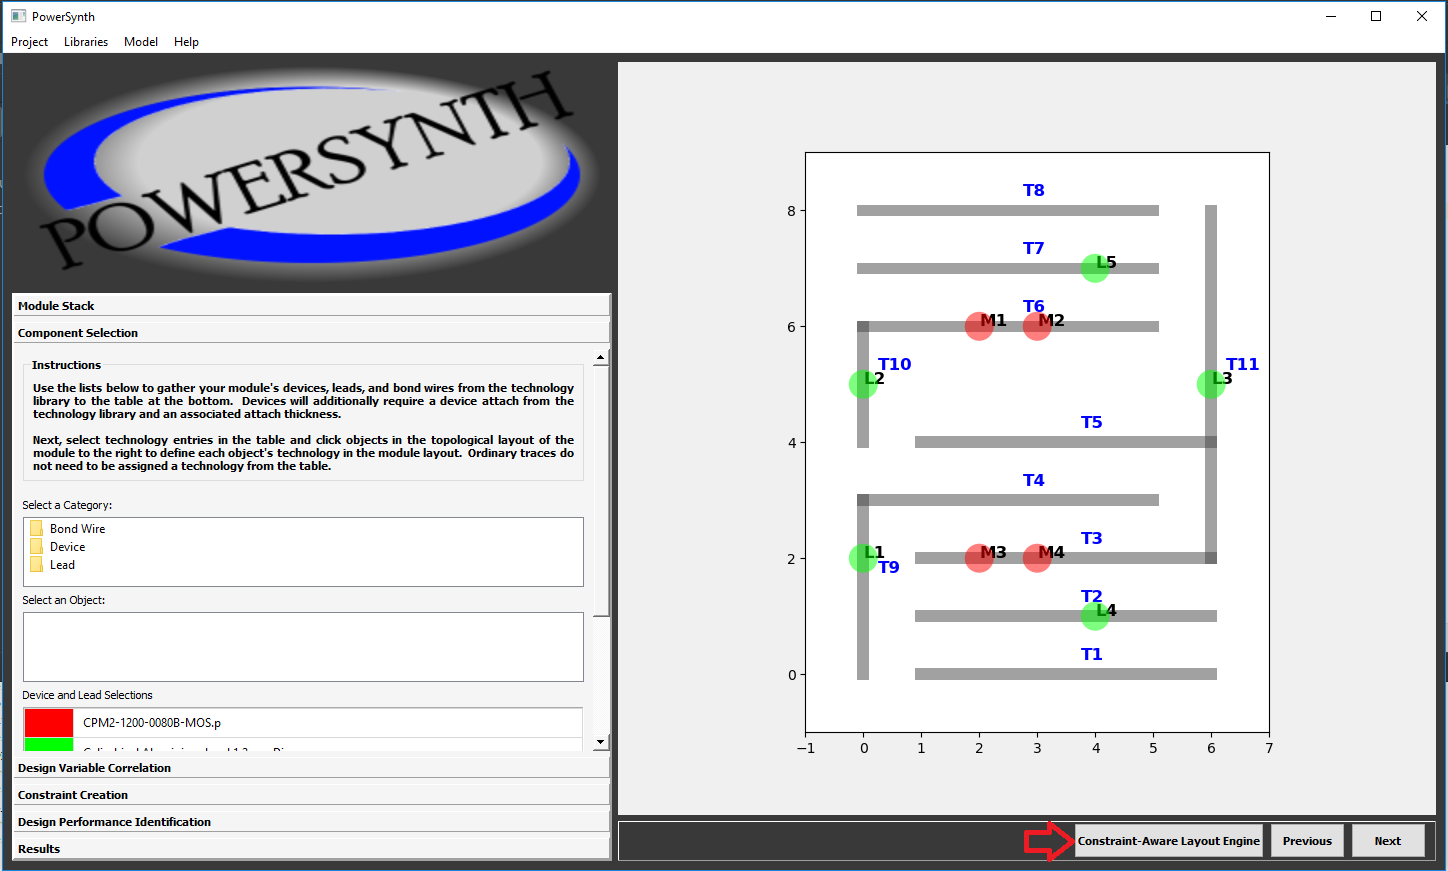
\includegraphics[width=0.9\textwidth]{./figs/start.PNG}
\caption{Entering into constraint-aware layout engine}
\label{start_w}
\end{figure}
\subsubsection{Constraint-Aware Layout Engine Dialog}
\label{sec-2-6-1}
The new window has four parts.
\begin{figure}[h]
\centering

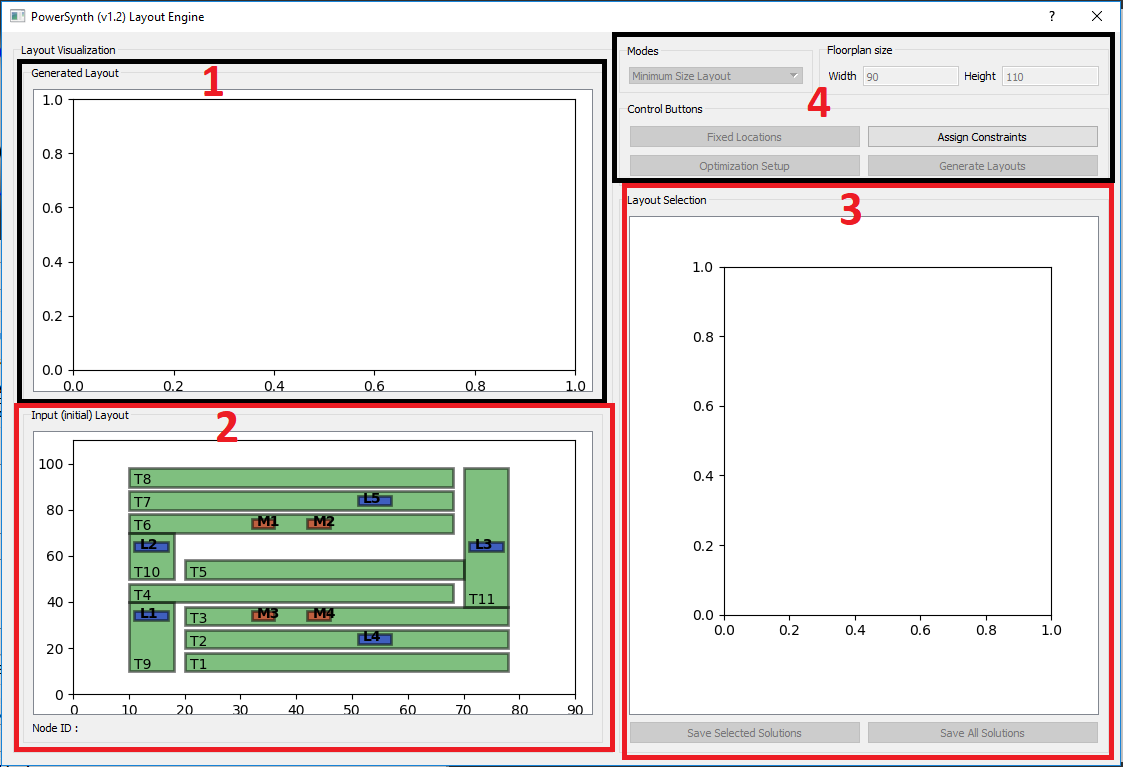
\includegraphics[width=0.9\textwidth]{./figs/new_dialog.PNG}
\caption{New Layout Engine Window}
\label{new_dialog}
\end{figure}
\begin{enumerate}
    \item \textbf{Generated Layout}: In this part, layout solution will be appeared.
    \item  \textbf{Input (Initial) Layout}: Here, the initial layout that is converted from symbolic layout will appear. This is just rectangular representation of the symbolic lines and points objects.
    \item  \textbf{Layout Selection}: This is the solution browser. Here, all solutions will be appeared as dots. Upon click on each dot corresponding layout will be shown in top left part (marked as 1 in the Fig.~\ref{new_dialog}).
    \item  \textbf{Control Features}: In this part, all information are shown and necessary input information are taken. Here, floorplan size of each layout, controlling features of the layout engine, different operating mode selection option are displayed.
\end{enumerate}

\subsubsection{Assign Constraints}
\label{sec-2-6-2}
At the starting of the constraint-aware layout engine, the constraints must be assigned. To assign constraints, the \textbf{“Assign Constraints”} button should be clicked and ‘Constraints setup’ window will appear (shown in Fig.~\ref{const}). There are four parts in the constraint setup: 1) Dimension Constraints, 2) Spacing Constraints, 3) Enclosure Constraints, and 4) Setup buttons. All constraints are automatically updated according to PowerSynth technology library. But the values can be modified by the user. Any modification can be performed in this table before clicking \textbf{"Apply to Layout"}.\\
\textbf{Setup Buttons}: After setting up the constraint values, to apply the constraints to the layout solutions \textbf{“Apply to layout”} button must be clicked. User can also load a constraint table from a csv file (in the same format shown in the Fig.~\ref{const}), by using \textbf{"Load DRC"} button. \textbf{"Save DRC"} button can be used to save the modified constraint table in csv format so that later it can be used.

\begin{figure}[t]
%\begin{center}
\centering

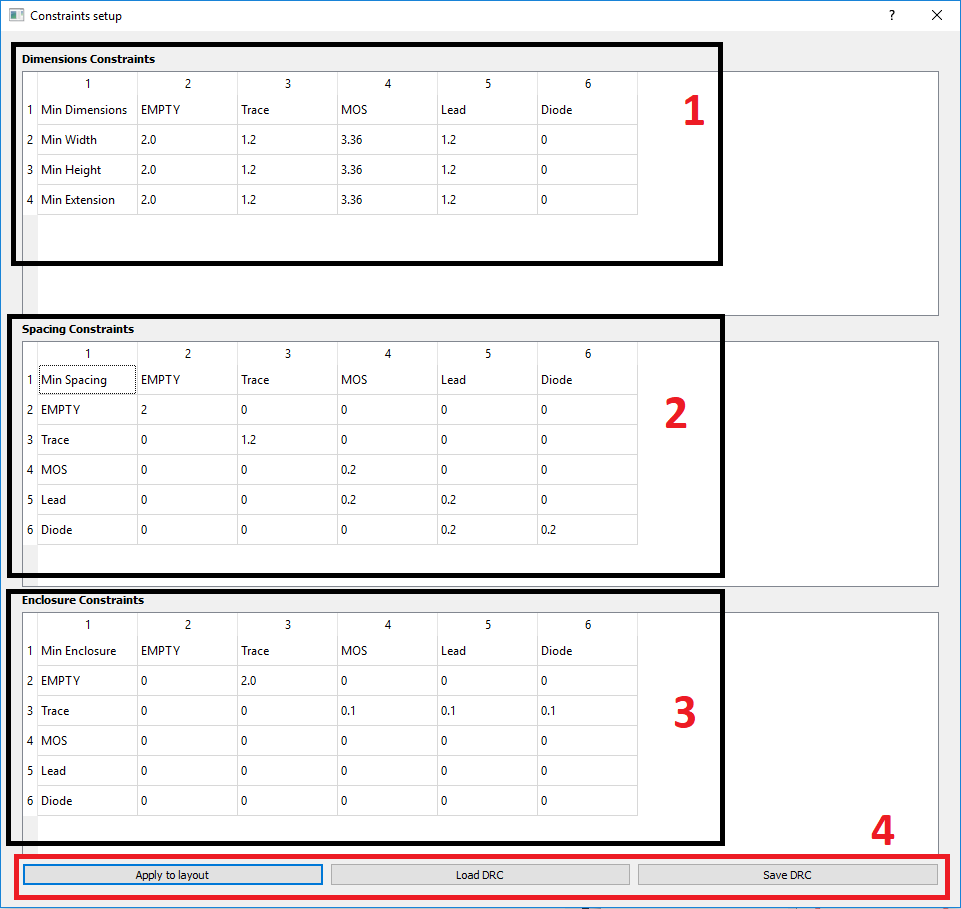
\includegraphics[width=0.9\textwidth]{./figs/cons_assign.PNG}
\caption{Constraint Table}
\label{const}
\end{figure}

Assign constraints is the first and the most important part for the layout engine. Without performing this step, layout solution generation is impossible.

\subsubsection{Modes}
\label{sec-2-6-3}
 To select the mode of operation, the drop down list under \textbf{“Modes”} can be used. The list is shown in Fig.~\ref{modes}. According to choice of the user the proper \textbf{"Mode"} should be selected, before generating layout.
\begin{figure}[t]
\centering
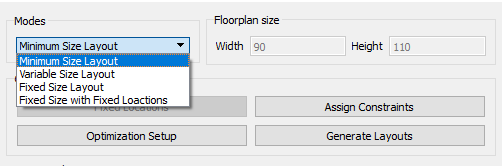
\includegraphics[scale=1]{./figs//modes.PNG}
\caption{Modes}
\label{modes}
\end{figure}

\begin{figure}[t]
\centering
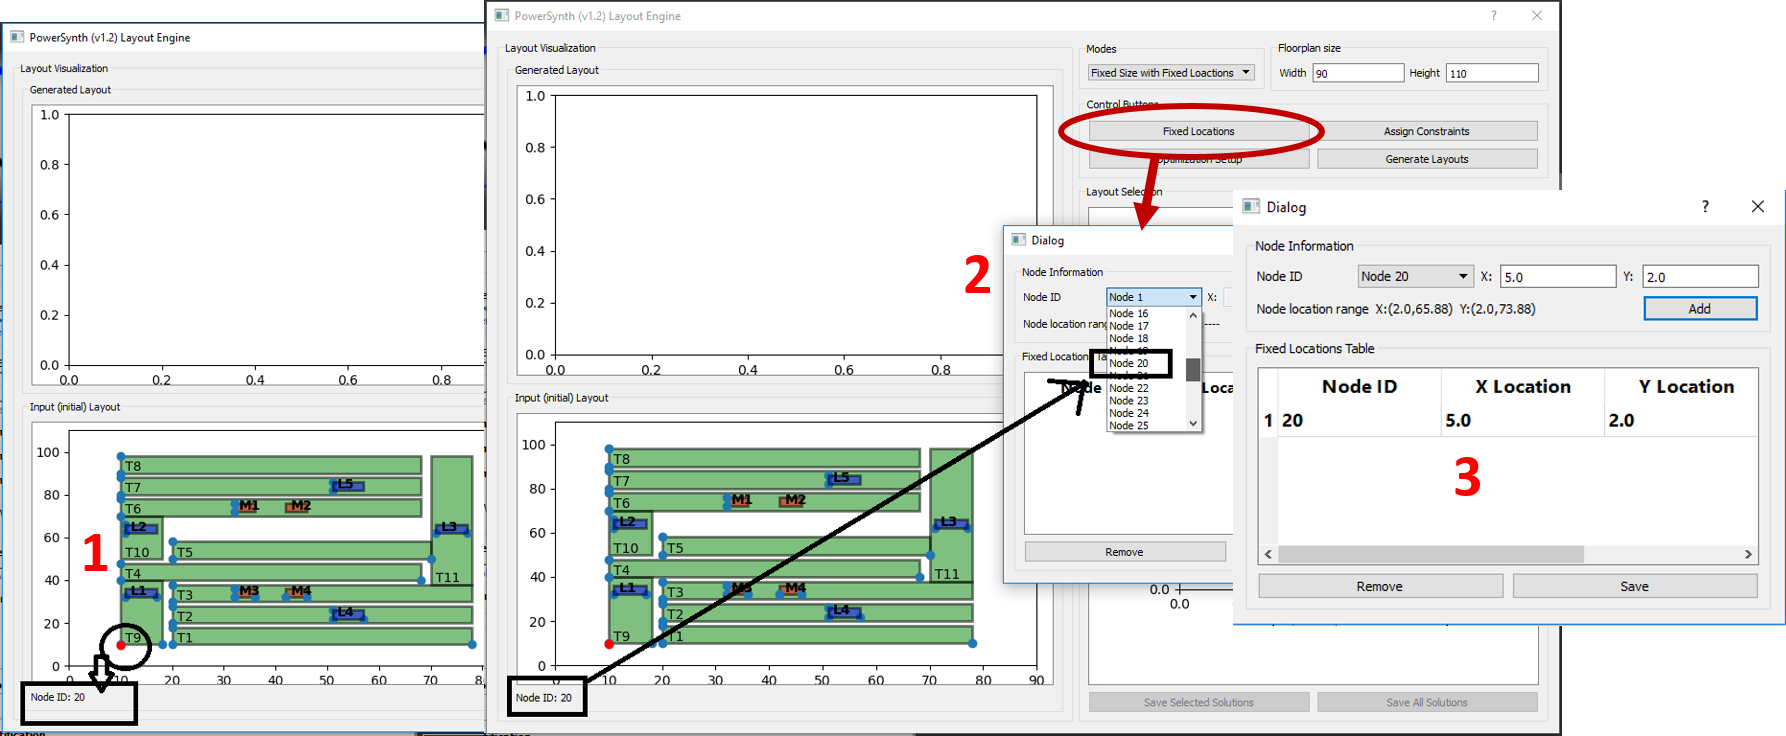
\includegraphics[width=1\textwidth]{./figs/Fixed_loc.png}
\caption{Fixed Location Setup}
\label{fix_loc}
\end{figure}

\begin{itemize}
    \item \textbf{Minimum Size Layout}: In this mode, only one layout will be generated. So, in the \textbf{"Optimization Setup"} option, only "Design Performance List" should be populated.
    \item \textbf{Variable Size Layout}: In this mode, user can generate arbitrary number of layouts. So, in the \textbf{"Optimization Setup"} option, along with "Design Performance List", \textbf{"Number of Layouts"} and \textbf{"Seed"} need to be provided.
    \item \textbf{Fixed Size Layout}: To have fixed floorplan sized layout solutions, user should enter \textbf{“Width”} and \textbf{“Height”} corresponds to floorplan size of the generated layouts. In this mode, user can choose \textbf{"Optimization Algorithm"}. If "NSGAII" is selected \textbf{"Number of Generations"} needs to be given, otherwise \textbf{"Number of Layouts"} needs to be provided. Also, \textbf{"Seed"} is a must.
    \item \textbf{Fixed Size with Fixed Locations}: In this mode,\textbf{“Width”}, \textbf{“Height”} must be given. Besides, one additional requirement is the \textbf{“Fixed Locations”}.This button is used for allocating fixed coordinates to the desired nodes. On this mode, the input layout is updated with clickable dots on possible nodes of the layout as shown in Fig.~\ref{fix_loc} with marked as "1". To fix a node at certain coordinate, user needs to click on the node and the \textbf{"Node ID"} will appear at the bottom. Then, \textbf{“Fixed Locations”} button needs to be clicked to find the desired "Node ID". Upon selecting the "Node ID" from the drop down list, the valid x and y coordinate range will appear for that node. User needs to choose a value within the range and then \textbf{"Add"} button needs to be clicked to store the location. In the similar way, as much nodes as user want can provide fixed location and then \textbf{"Save"} button needs to be clicked to apply the location values to the generated layout. A flow is shown in Fig.~\ref{fix_loc}
\end{itemize}

At a time one mode of operation should be selected to generate solution.
How to perform different mode operations is shown in the later part using an example.

\subsubsection{Optimization Setup}
\label{sec-2-6-4}
To generate layout solution, the performance metrics should be chosen. To setup the measurement metrics \textbf{"Optimization Setup"} button needs to be clicked and a dialog (shown in Fig.~\ref{opt_setup}) will appear.
\begin{figure}[H]
%\begin{center}
\centering

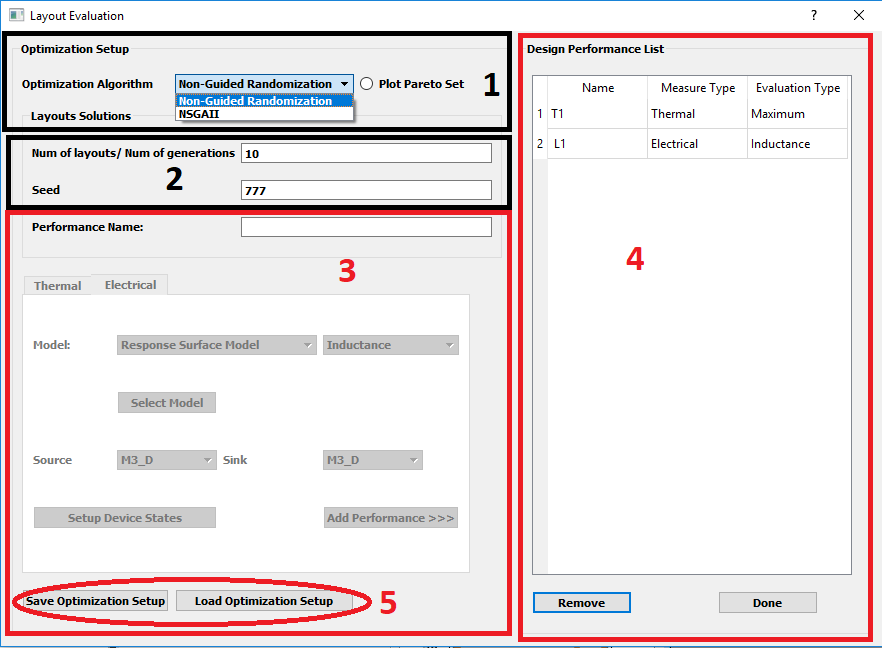
\includegraphics[width=0.9\textwidth]{./figs/optimization_setup.PNG}
\caption{Optimization Setup Dialog}
\label{opt_setup}
\end{figure}

There are five parts of this dialog.
\begin{enumerate}
    \item \textbf{Optimization Setup}: Here, there are two options for choosing an optimization algorithm: 1) Non-Guided Randomization, and 2) NSGAII. Currently, NSGAII is only available for \textbf{Fixed Size Layout} generation mode. The radio button should be checked for plotting the Pareto-front only otherwise the whole solution sets will be appeared on the solution browser.
    
    \item \textbf{Layout Solutions}: For NSGAII, the number of generations and randomization seed should be provided, whereas for the non-guided randomization, the total number of layouts to be generated and seed need to be provided for all modes of layout generation except the \textbf{Minimum Size Layout} case.
    
    \item \textbf{Performance Metrics Information}: In this version, two types of measurements are included: electrical (loop inductance, capacitance, and resistance) and thermal (maximum, average, and std. deviation). The measurement setup is similar to the steps described in \ref{sec-2-5}.
    
    \item \textbf{Design Performance List}: After describing each performance (i.e., electrical, thermal), upon clicking on the \textbf{"Add Performance"} button this list will be populated. In this version, at a time only two performance metrics can be chosen as the 3-D solution browser is not integrated in the beta-version.
    
    \item \textbf{Save and Load Optimization Setup}: For a certain project, user can save optimization setup by clicking on \textbf{"Save Optimization Setup"} button just after declaring all design performances. Later, for the same project, user can load the saved optimization setup file using the button \textbf{"Load Optimization Setup"}.
\end{enumerate}

\subsubsection{Generate Layouts}
\label{sec-2-6-5}
After completing each step stated above the \textbf{“Generate Layouts”} button should be clicked to generate solutions. Upon clicking this button, in the solution browser, solutions will appear as dots (shown in Fig.~\ref{gen_layout}). In the figure, the red dot corresponding layout is appeared in the \textbf{Layout Visualization} section of the window. Upon clicking on each dot, the corresponding layout will appear there. As the widths and heights of all rectangles are varied, the devices and leads may not have a fixed dimension in the generated solutions. So, in the generated layout, the dotted lines show the possible room for that device or lead and the component is placed at the center of that room.
\begin{figure}[t]
%\begin{center}
\centering
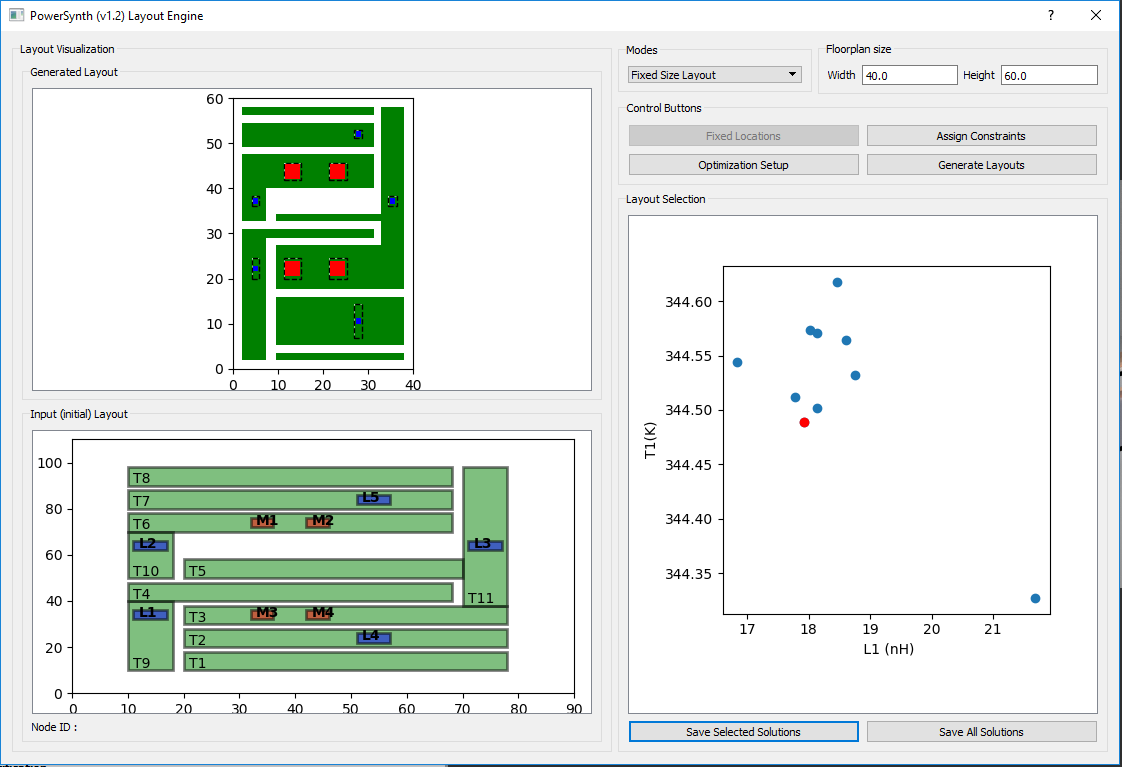
\includegraphics[width=0.9\textwidth,height=3.8 in]{./figs/gen_layout_env.PNG}
\caption{Generate Layouts}
\label{gen_layout}
\end{figure}
\subsubsection{Saving Solutions}
\label{sec-2-6-6}
 After layout generation, user can save each selected solution in the main window of PowerSynth by using \textbf{"Save Selected Solution"} button for further export operations (shown in Fig.~\ref{save_sol}). Also, all solution information can be saved as csv format upon clicking on the button \textbf{"Save All Solutions"}. In this case, for each solution, one csv file will be created having all performance values and layout information. Also, another csv file will save all performance data only.

 \begin{figure}[H]
%\begin{center}
\centering
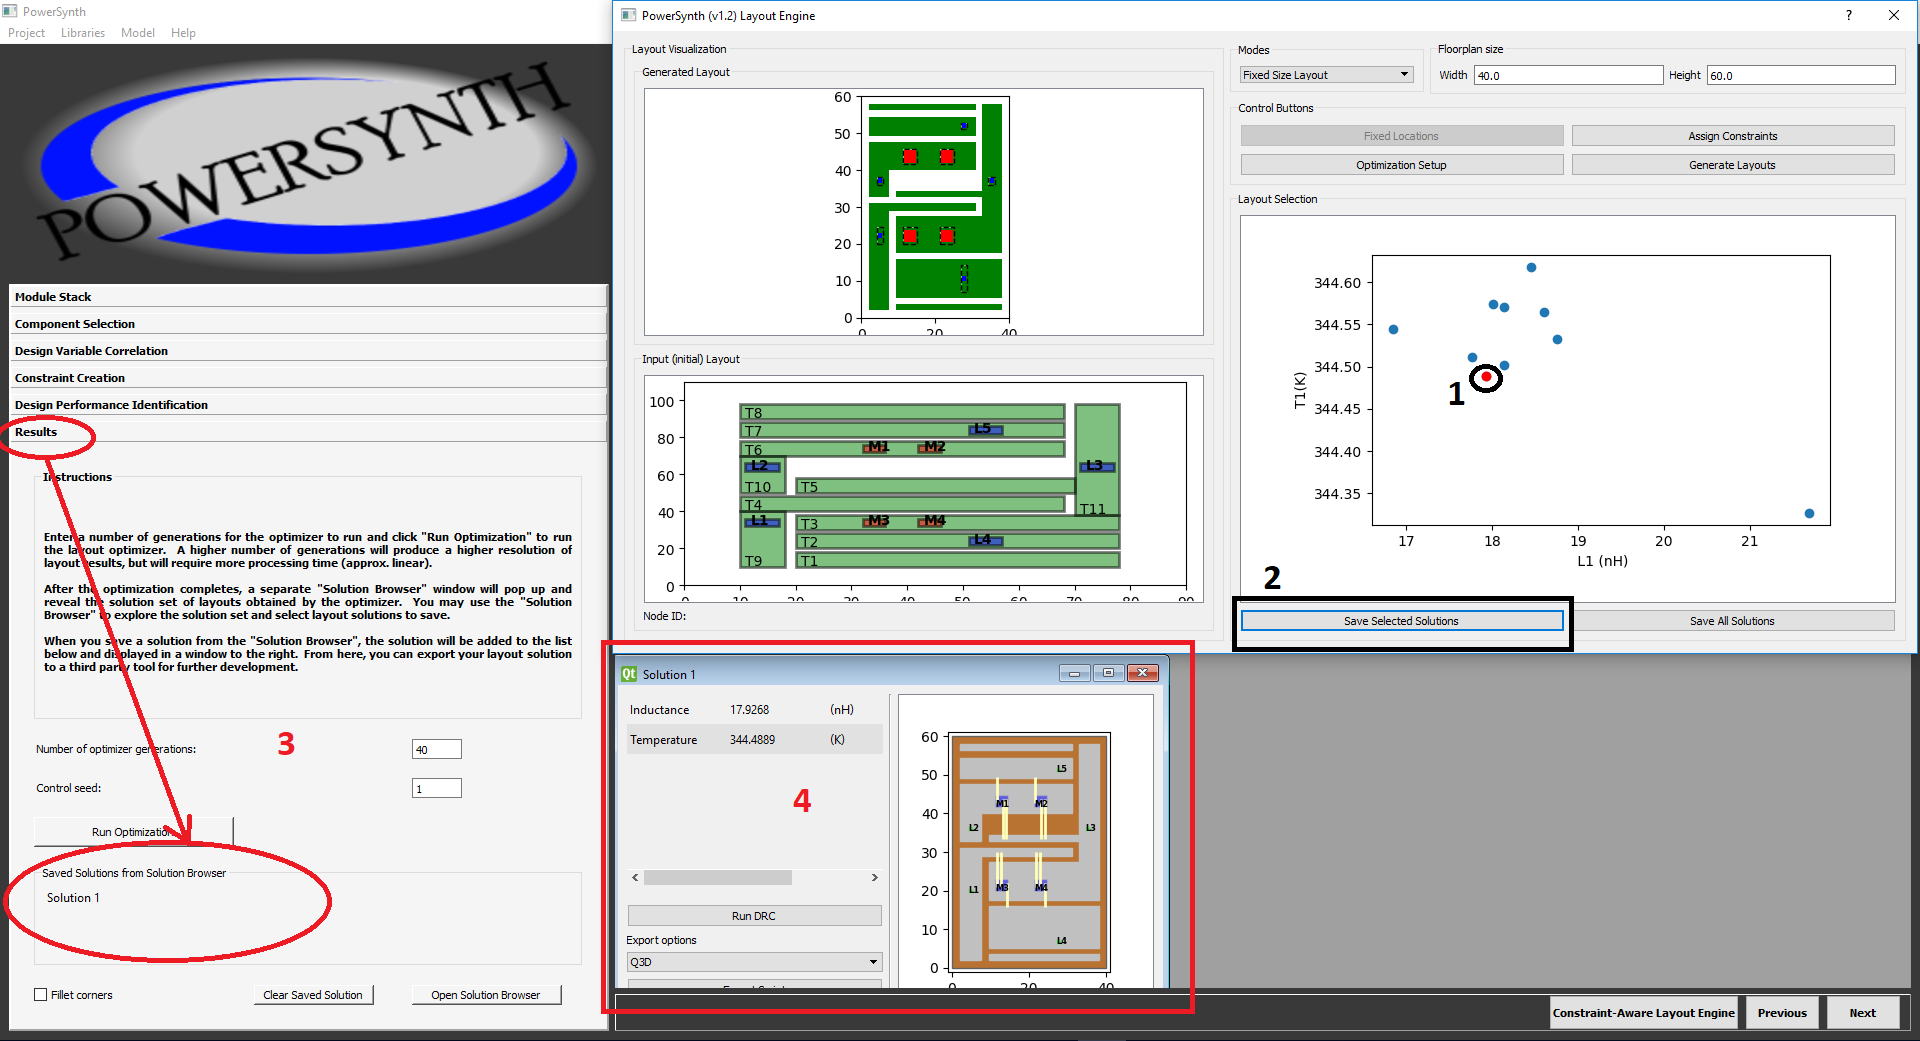
\includegraphics[width=0.9\textwidth, height=4 in]{./figs/Saving_sol.PNG}
\caption{Saving Selected Solution}
\label{save_sol}
\end{figure}

\subsubsection{Test Case}
\label{sec-2-6-7}
The same case described in \ref{sec-2-2} is used for testing the new layout engine. The whole flow is shown sequentially.

To use new layout engine the input script must be in the same format described in  \ref{sec-2-2}. The name of the component must start with first letter of the component name (i.e., Trace--> T, MOSFET--> M, Lead--> L, and Diode--> D). In this version these four components are allowed to place in the floorplan.

Before clicking on the \textbf{"Constraint-Aware Layout Engine"} button user must complete each steps up to \textbf{"component selection"}. After that upon clicking on \textbf{"Constraint-Aware Layout Engine"} button the updated layout engine dialog will appear (shown in Fig.~\ref{test_new_dialog}).
\begin{figure}[H]
\centering
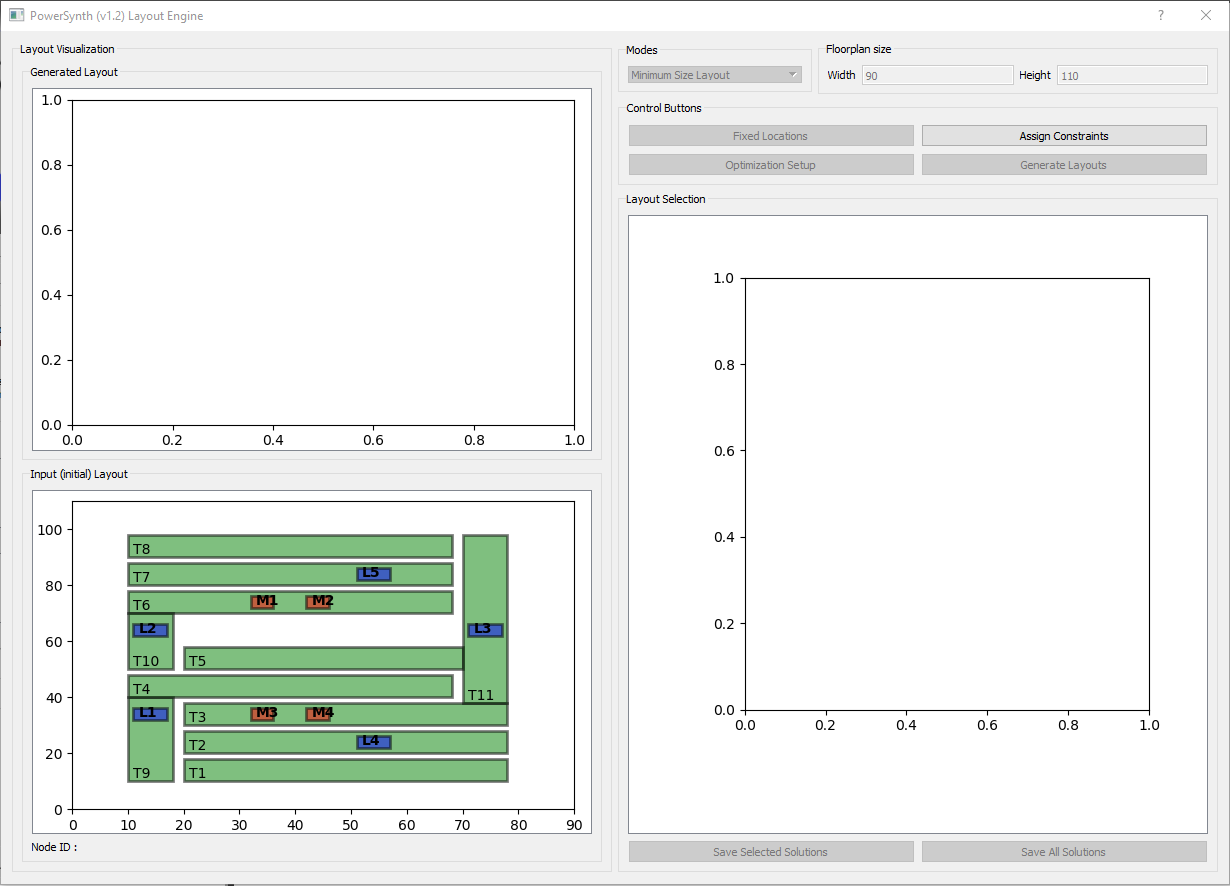
\includegraphics[width=0.9\textwidth]{./figs/Test/start.PNG}
\caption{Constraint-Aware Layout Engine Dialog}
\label{test_new_dialog}
\end{figure}


At this stage, only \textbf{"Assign Constraints"} button is enabled. Click on the button and the constraint setup window (Fig.~\ref{cons}) will appear.
\begin{figure}[t]
\centering
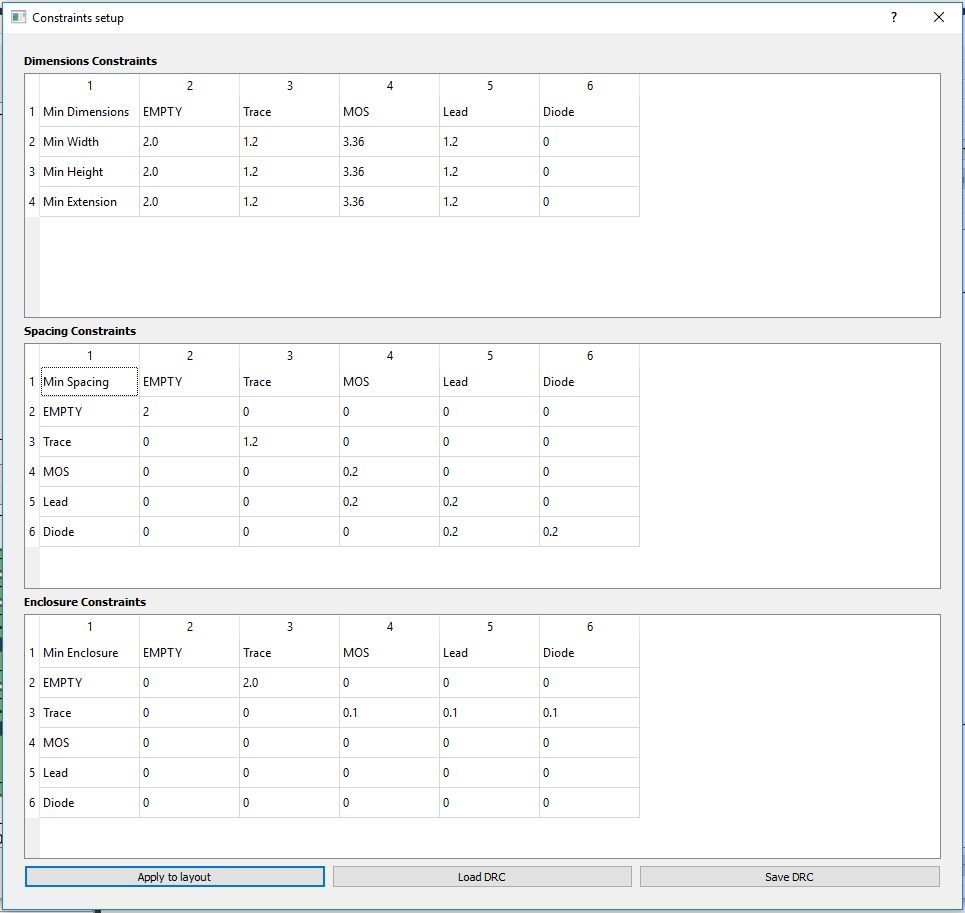
\includegraphics[width=0.9\textwidth]{./figs/Test/constraint.PNG}
\caption{Constraint Table}
\label{cons}
\end{figure}

The constraint values are already inserted from technology library, so just click on the \textbf{"Apply to Layout"} button to implement the constraints.

Now, a mode of operation needs to be selected.

\begin{itemize}
    \item \textbf{Mode 0: Minimum Size Layout}\\
    Choose \textbf{"Minimum size Layout"} from the drop down list on the "Modes" section. Then click on the \textbf{"Optimization Setup"} button to add performance metrics. Upon clicking the button, the optimization setup window will appear (shown in Fig.~\ref{opt_set_mode_0}). Initially, only \textbf{"Performance Name"} field is editable as rest of them are fixed for Mode 0. Here, for thermal evaluation "T1" is entered as "Performance Name" and then click on the "Thermal" tab to choose thermal model and evaluation type. In this case, "FEM" model is chosen and "Maximum" temperature is picked for measurement. Then mark the check boxes corresponding the devices you want to measure. Here, all devices are considered. Then click on the \textbf{"Add Performance"} button to store the thermal measurement configuration in the "Design Performance List". Then again, the \textbf{"Performance Name"} field is populated with "L1" to measure inductance for the layout. Click on the "Electrical" tab to define electrical performance parameters. First, Model (Micro strip) and then type of measurement (Inductance) are chosen. In case of "Response Surface Model", \textbf{"Select Model"} button needs to be used to implement the model. Now, to calculate loop inductance one source and sink from the layout are chosen. In this example source is "L5" and sink is "L4". Then to complete the loop, \textbf{"Setup Device States"} button needs to be used to add proper connection (similar to shown in \ref{sec-2-5-4}). Having all of the setup click on the \textbf{"Add Performance"} button to add the measurement in the "Design Performance List". After each step the window status is shown in Fig.~\ref{opt_set_mode_0}. Now click on the \textbf{"Done"} button. Also, the optimization setup can be saved by clicking on \textbf{"Save Optimization Setup"} button. Later the same setup file can be loaded for this case using the button \textbf{"Load Optimization Setup"}.
    \begin{figure}[t]
    \centering
    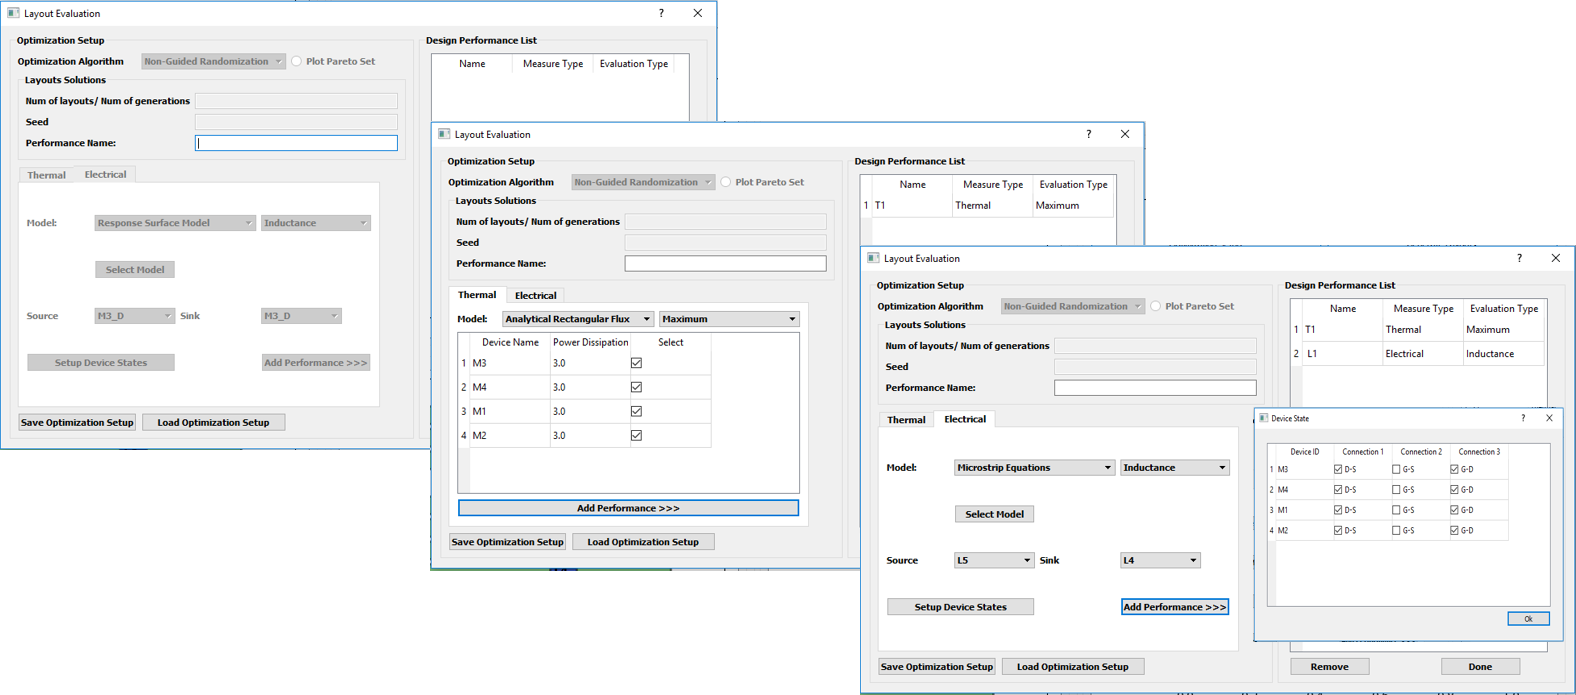
\includegraphics[width=0.9\textwidth]{./figs/Test/Picture1.png}
    \caption{Mode 0 optimization setup flow}
    \label{opt_set_mode_0}
    \end{figure}
     After adding performances, click on the \textbf{"Generate Layouts"} button to have the minimum size layout. It will show one dot in the "Layout Selection" frame. Upon clicking on the dot, the \textbf{"Width"} and \textbf{"Height"} field will be populated with minimum size of the solution and "Generated Layout" frame will show the layout. The result is shown in Fig.~\ref{mode_0_sol}.
     
    \begin{figure}[H]
    \centering
    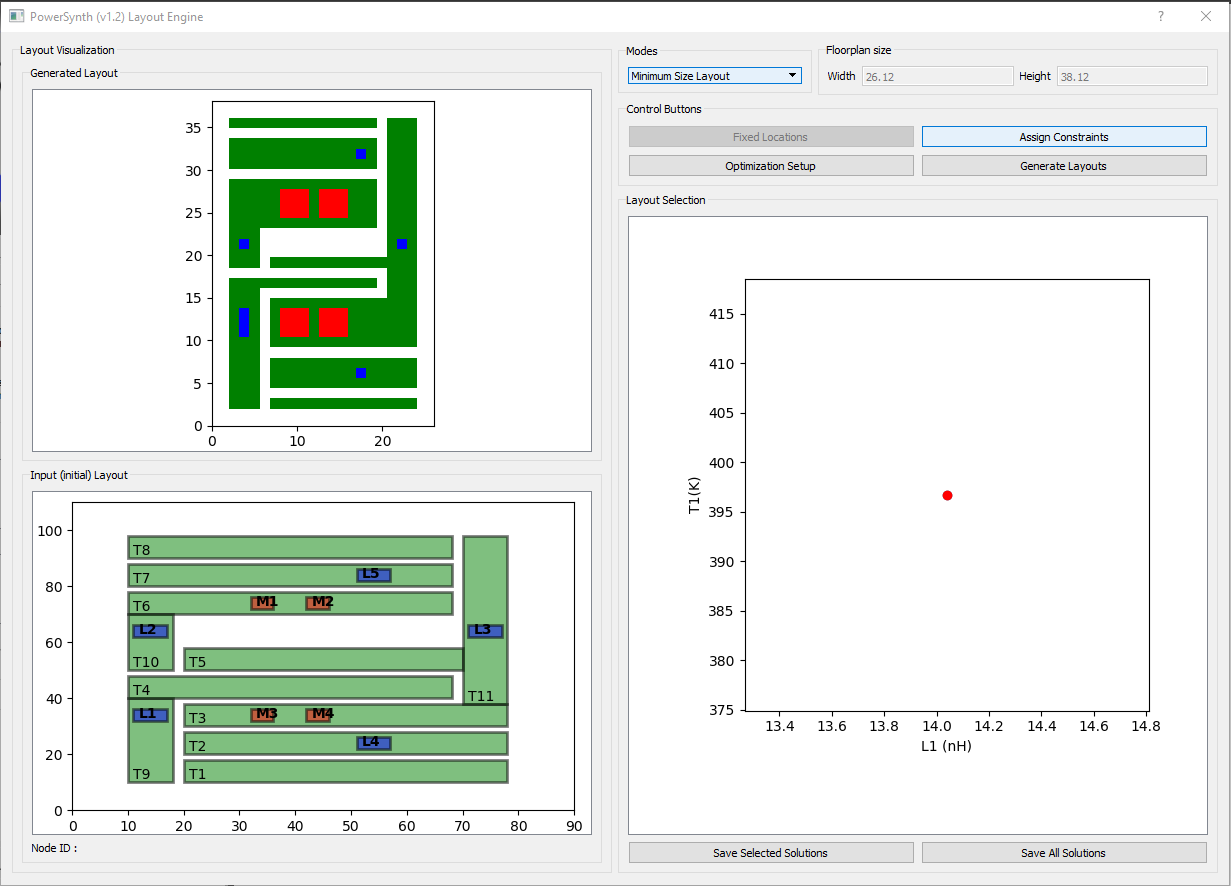
\includegraphics[width=0.9\textwidth, height=3.5 in]{./figs/Test/Mode_0_sol.PNG}
    \caption{Minimum size Layout Solution}
    \label{mode_0_sol}
    \end{figure}
    
    Using \textbf{"Save Selected Solutions"} button, the solution can be saved to main window (shown in Fig.~\ref{save_sol} (a)) and using \textbf{"Save All Solutions"} button, the data can be saved to a csv file (shown in Fig.~\ref{save_sol} (b)).
    \begin{figure}[t]
    \centering
    \subfloat[Solution in main window]{{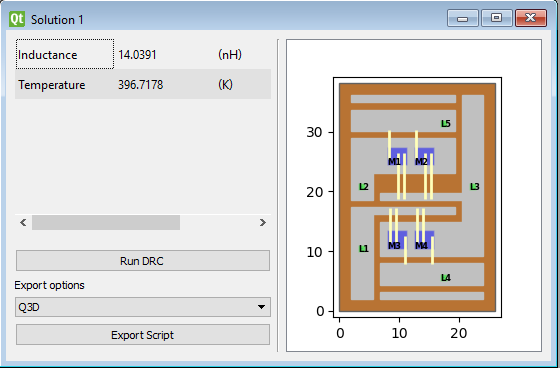
\includegraphics[width=7cm, height=2in]{./figs/Test/sol_main.png} }}%
    \qquad
    \subfloat[Layout data in csv]{{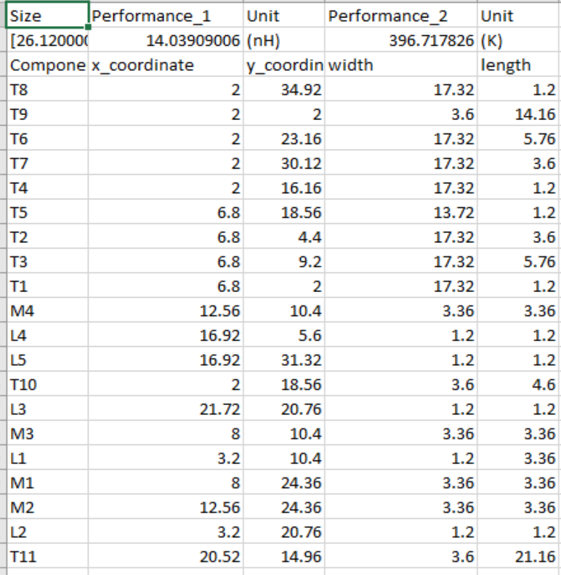
\includegraphics[width=7cm, height=2in]{./figs/Test/csv.PNG} }}%
    \caption{Saving solution options}
    \label{save_sol}
    \end{figure}
    \item \textbf{Mode 1: Variable Size Layout}\\
    To produce variable floorplan size layout solutions, select the \textbf{"Variable Size Layout"} from the drop down list on the "Modes" section. Now, click on the \textbf{"Optimization Setup"} button to input the "Number of layouts" to be generated and a randomization "Seed" in the corresponding fields. As performance metrics are already setup for this case, don't need to update that again. At this stage the "Optimization Setup" window will look like the same as shown in Fig.~\ref{mode_1_opt}.Also, to get the PAreto-front of the solutions, \textbf{"Plot Pareto Set"} can be checked.
    
    \begin{figure}[t]
    \centering
    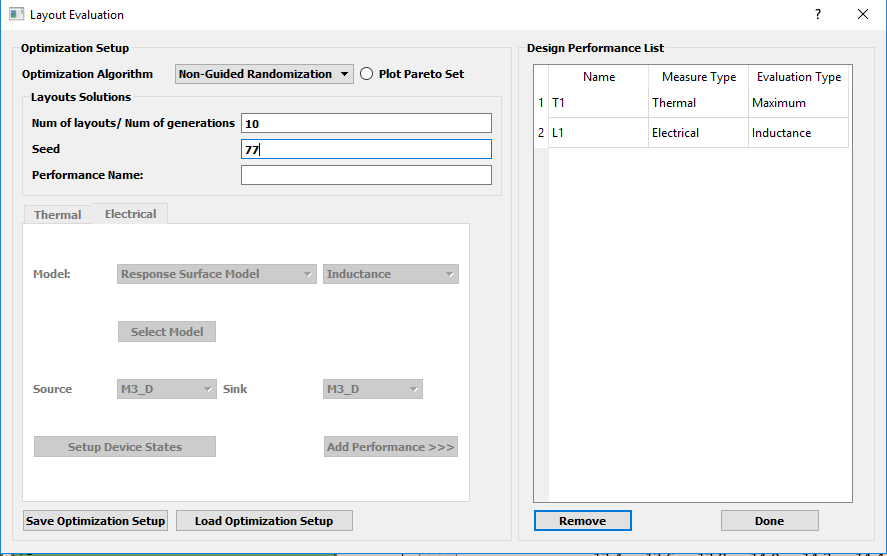
\includegraphics[width=0.9\textwidth]{./figs/Test/Mode_1_opt_setup.PNG}
    \caption{Mode 1 optimization setup}
    \label{mode_1_opt}
    \end{figure}
     Then click on the \textbf{"Generate Layouts"} button to generate 10 solutions. The result will appear on the solution browser and upon clicking on different dots, corresponding layout is shown in the "Generated Layout" frame. Also, "Width" and "Height" of the corresponding layout is shown in those fields. A sample layout is shown in Fig.~\ref{mode_1_sol}. After getting all solutions, using the \textbf{"Save Selected Solutions"} button and \textbf{"Save All Solutions"} button those solutions can be exported.
     
    \begin{figure}[t]
    \centering
    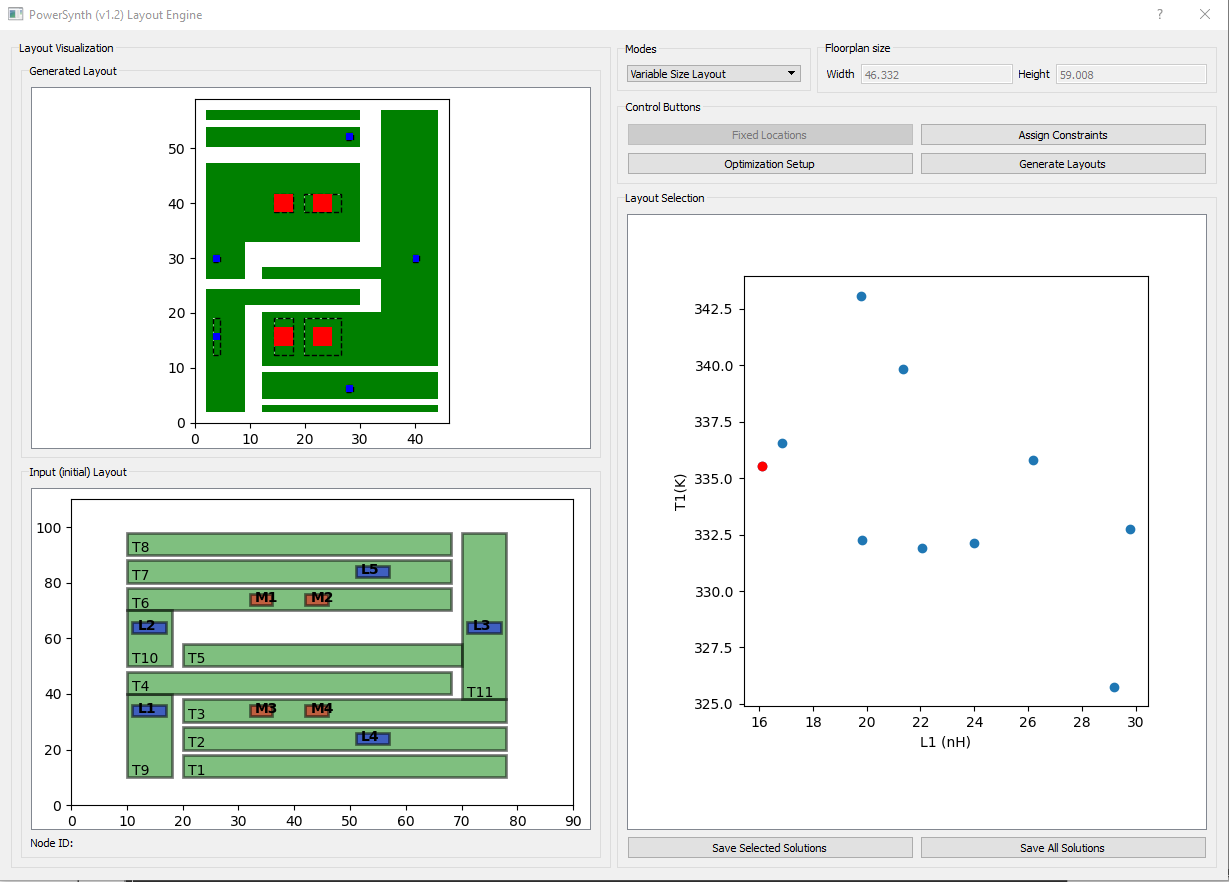
\includegraphics[width=0.9\textwidth]{./figs/Test/mode_1_sol.PNG}
    \caption{Mode 1 solution}
    \label{mode_1_sol}
    \end{figure}
    \item \textbf{Mode 2: Fixed Size Layout}\\
    Upon choosing this mode from the "Modes" options, the floorplan size needs to be provided in \textbf{"Width"} and \textbf{"Height"} fields. Then in the "Optimization Setup", there are two options: 1) Non-Guided Randomization and 2) NSGAII. For the first option, "Number of Layouts", and for the second option "Number of Generations" needs to be provided along with the "Seed". The setup looks like the Fig.~\ref{mode_2_opt}. Now, after clicking the \textbf{"Done"} button,\textbf{"Generate Layouts"} button can be clicked. A new set of solutions will be appeared (shown in Fig.~\ref{mode_2_ng}). Now, for NSGAII as "Optimization Algorithm" with 100 generations and seed=77, the solution set is shown in the Fig.~\ref{save_sol_NSGAII}(a) and corresponding Pareto-front is shown in the Fig.~\ref{save_sol_NSGAII}(b).
    
    \begin{figure}[H]
    \centering
    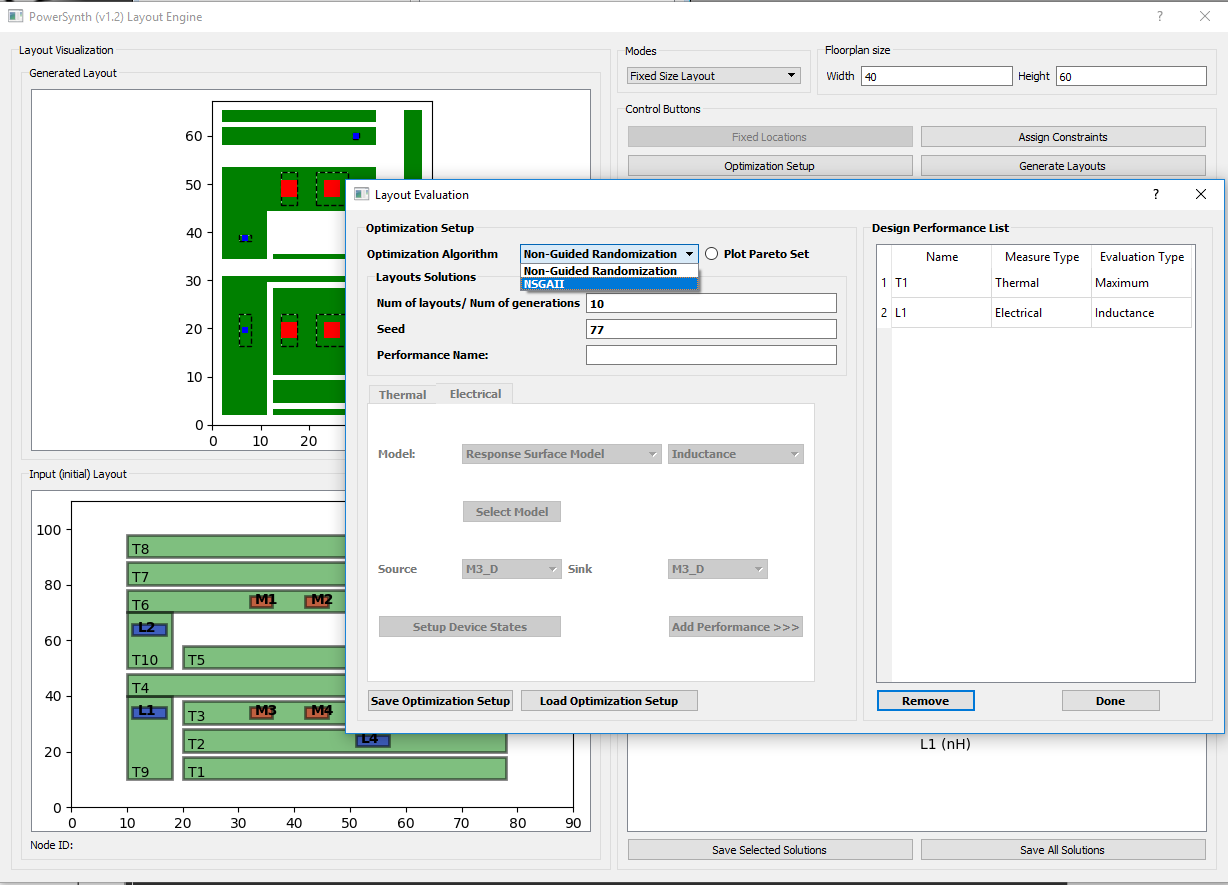
\includegraphics[width=0.9\textwidth]{./figs/Test/Mode_2_opt.PNG}
    \caption{Mode 2 optimization setup}
    \label{mode_2_opt}
    \end{figure}
    
    \begin{figure}[t]
    \centering
    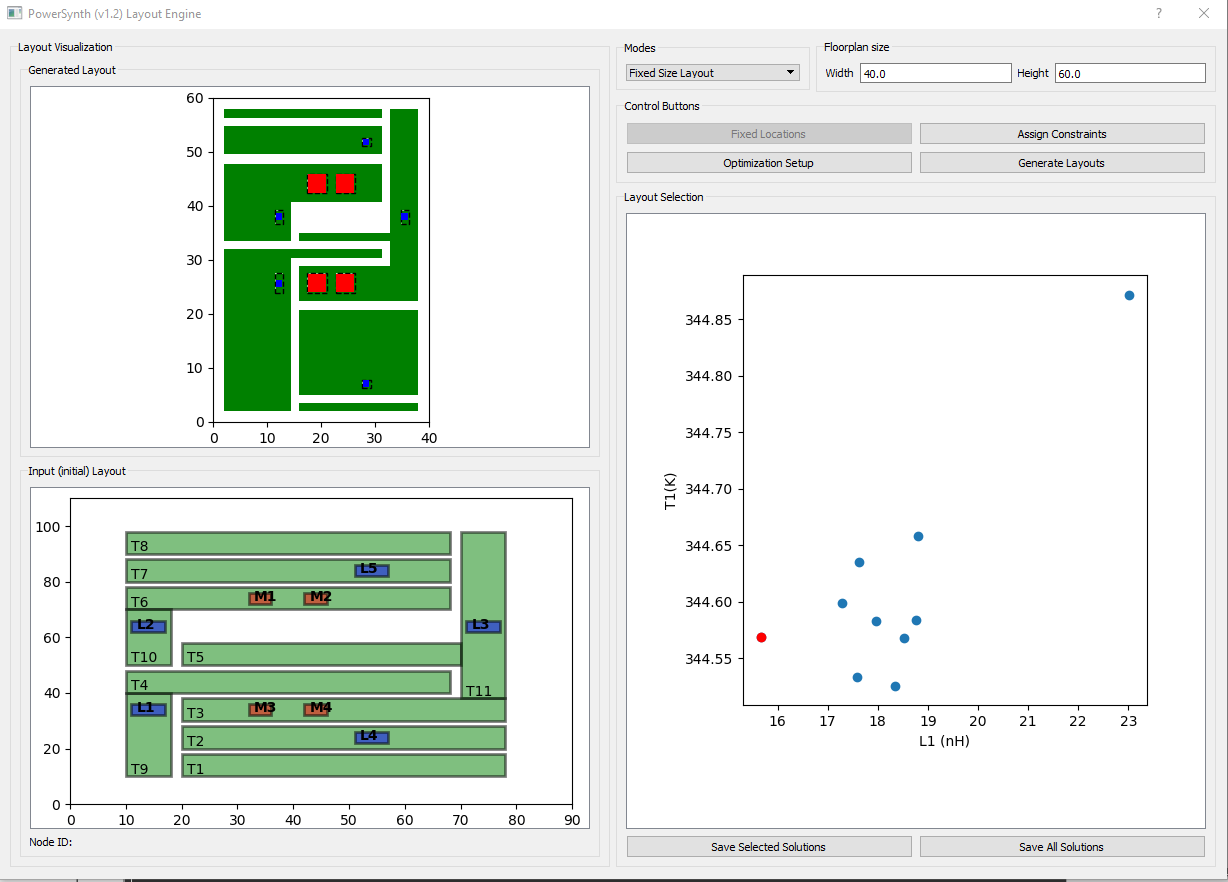
\includegraphics[width=0.9\textwidth]{./figs/Test/Mode_2_NG.PNG}
    \caption{Non-Guided Randomization Solutions}
    \label{mode_2_ng}
    \end{figure}
    
    \begin{figure}%
    \centering
    \subfloat[Solution set for NSGAII]{{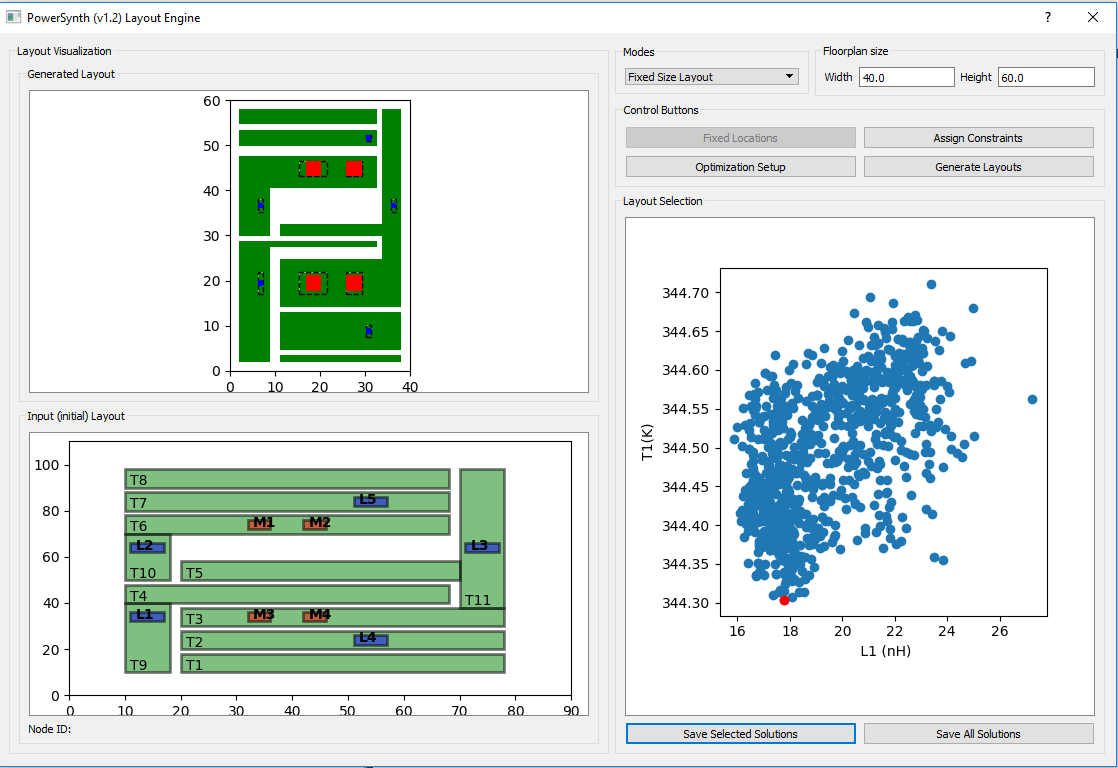
\includegraphics[width=7.5cm, height=2.5in]{./figs/Test/NSGAII.PNG} }}%
    \qquad
    \subfloat[Pareto-front of (a)]{{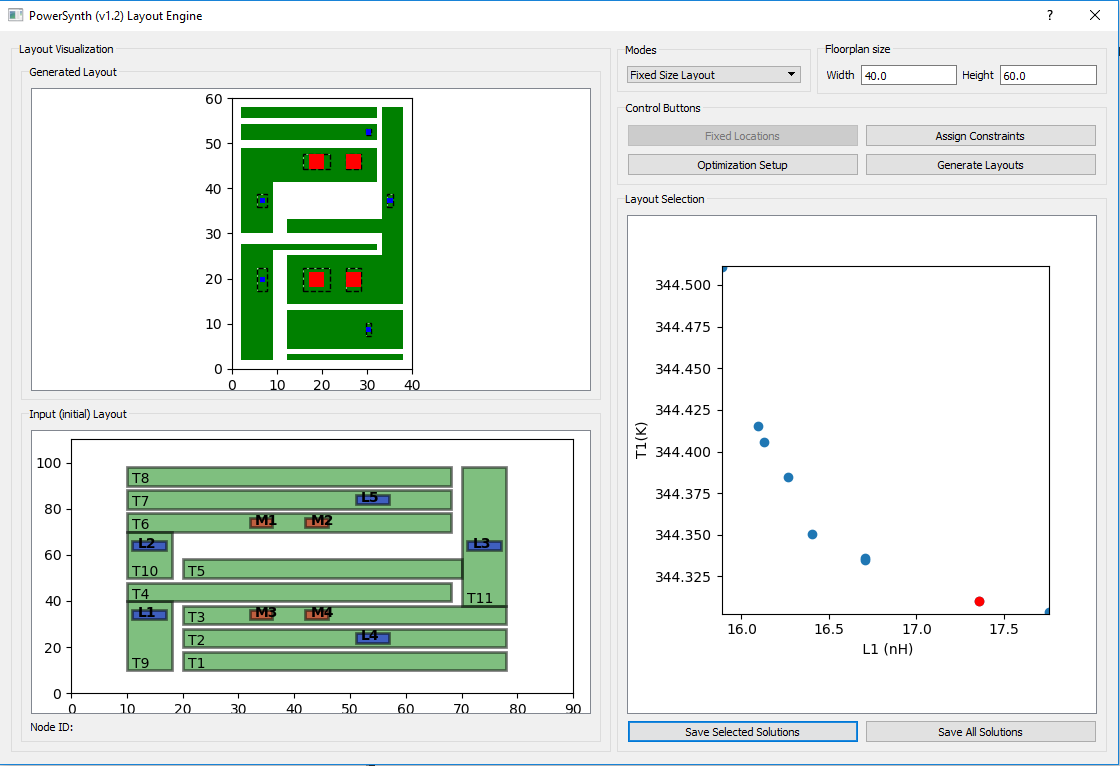
\includegraphics[width=7.5cm, height=2.5in]{./figs/Test/Pareto.PNG} }}%
    \caption{Mode 2 optimization results for NSGAII}
    \label{save_sol_NSGAII}
    \end{figure}
    \item \textbf{Mode 3: Fixed Size with Fixed Locations}\\
    In this mode of operation, let's fix the leads "L4", and "L5" at certain x locations and leads "L2", and "L3" at certain y locations as shown in the table. as "L4", "L5" are correlated vertically and "L2","L3" are correlated horizontally, between two of them, we need to fix one.
    
    \begin{table}[H]
    \centering
    \caption{Desired fixed location of Leads}
    \label{tab:my-table}
    \begin{tabular}{|c|c|c|c|}
    \hline
    \textbf{Components} & \textbf{x-location} & \textbf{Components} & \textbf{y-location} \\ \hline
    L4, L5 & 28 & L3, L2 & 40 \\ \hline
    \end{tabular}
    \end{table}
    
    To setup locations according to the table, after selecting \textbf{" Fixed Size with Fixed Locations"} mode from the "Modes" click on the \textbf{"Fixed Locations"} button. Then map desired "Node ID" from the layout to the fixed location table. The table should look like the Fig.~\ref{fix_loc_set}. Then click the \textbf{"Save"} button to store the given locations. The optimization setup is kept same as Mode 2 with non-guided randomization.
    \begin{figure}[H]
    \centering
    \includegraphics[width=0.9\textwidth]{./figs/Test/mode_3_fix.PNG}
    \caption{Fixed location setup}
    \label{fix_loc_set}
    \end{figure}
     Upon clicking on \textbf{"Generate Layouts"} button the solution set will appear in the solution browser and look like the Fig.~\ref{mode_3_res}. Follow the dotted lines coordinate to find the match of the coordinates. In all of the solutions "L3" and "L2" have y-coordinate of 40, "L4" and "L5" have x-coordinate of 28.
     
     \begin{figure}[H]
    \centering
    \includegraphics[width=0.9\textwidth]{./figs/Test/mode_3_result.PNG}
    \caption{Mode 3 solutions}
    \label{mode_3_res}
    \end{figure}
    
    
\end{itemize}

\pagebreak

\subsection{Optimization and Results}
\label{sec-2-6}

In this step, the user will need to specify number of generations. Since PowerSynth is based on a heuristic genetic algorithm, a higher number of generations will give you more solution choices. For this simple example 100 should be sufficient.

Click \textbf{Run Optimization.} The software will ask the user to save the project. Navigate to your specified project directory or any other directory to save this information. Note that the information from last run will be erased if it is not saved elsewhere. However, if the setup, number of generations, and the control seed (used for optimizer random generator) are kept the same, the final result will be the same. The runtime depends on number of generations specified. Upon completion, the solution window is opened as shown below.

\begin{center}
\includegraphics[width=0.7\textwidth]{./figs/26_Optimization.png}
\end{center}

Check the console for progress updates. Once the optimizer routine is over, a new window should appear. Check your task bar if the window does not pop up. This is what the window may look like (depending on your unique solutions). 

\begin{center}
\includegraphics[width=0.7\textwidth]{./figs/27_SolutionBrowser.png}
\end{center}

Left click and hold with your mouse inside the graph to rotate the graph. Choose the axes you wish to show using the pane on the left side (the scroll bar on the right will allow you to see more if they are not all visible). Each dot on the graph is a unique solution. Click on a solution and it will be colored red while displaying its preview on the left. Click on a different solution to see how the layout changes. The corresponding values for the objective functions are given below the layout preview. 

To save the entire solution set, use the Export Solution Set button and save in .csv format. You can use Excel to open the file. 

To save a solution for export into other tools or to see the E/T netlists, click on “Save Layout to Main Window.” You can enter a name for this solution. In this case it is “Solution 1.”

\begin{center}
\includegraphics[width=0.7\textwidth]{./figs/28_SolnBrowser.png}
\end{center}


Under “Saved Solutions from Solution Browser” you can see Solution 1. The solution interface allows the user to export the solution to Q3D or SolidWorks. Other options allow the user to obtain the thermal and electrical netlists. The “Run DRC” button allow user to validate the design vs the Process Design Rule. To validate against different Process Design Rules see the section detailing the Process Design Rules Editor.

\begin{center}
\includegraphics[width=0.6\textwidth]{./figs/29_SolnExport.png}
\end{center}

\pagebreak

\subsection{Post-Layout Optimization}
\label{sec-2-7}

PowerSynth allows the user to optionally apply corner correction to prevent electric field focusing and enhance thermo-mechanical reliability. 

To apply fillets, in the Results tab, one may either check the ‘Fillet corners’ box, open the solution browser, and then select and save a solution, or alternatively, check the ‘Fillet corners’ box, and double click an existing solution under the ‘Saved Solutions from Solution Browser’ section to apply the fillets to an existing solution.
For example, before applying fillets to solution 4:

\begin{center}
\includegraphics[width=0.7\textwidth]{./figs/41_PL1.png}
\end{center}

And after applying fillets to solution 4, a new sub-window with the filleted solution appears:

\begin{center}
\includegraphics[width=0.7\textwidth]{./figs/42_PL2.png}
\end{center}

The arrow pointing up shows the same solution without fillets at the tail and with fillets at the head. 

\begin{center}
\includegraphics[width=0.6\textwidth]{./figs/43_PL3.png}
\end{center}

\pagebreak

\subsection{Exporting Saved Solutions}
\label{sec-2-8}

\subsubsection{Export to ANSYS Q3D}
\label{sec-2-8-1}

Select \texttt{Q3D} from the export options list.Choose a directory, and create a file name. This will generate a .vbs file. In ANSYS Q3D open a new Q3D project. Go to \textbf{Tool-> Run Script} and load the exported .vbs file , the result is shown as below.

\begin{center}
\includegraphics[width=0.7\textwidth]{./figs/30_Q3D.png}
\end{center}

\subsubsection{Export to SolidWorks}
\label{sec-2-8-2}

Choosing this option will open a dialog is asking the user for their SolidWorks version. After typing the version (e.g. 2016) for the SolidWorks. Hit ok and choose an output directory. A*.swp file is exported. However, this is not a binary file and can be somewhat troublesome to run thisscript. In SolidWorks, under Tools-> Macro select “New” (do not choose edit or run since the *.swp from PowerSynth is just a text file, not binary). Copy and paste the text from the exported SolidWorks file and paste into the macro code editor. Finally press “RUN” (green triangular button).

\begin{center}
\includegraphics[width=0.7\textwidth]{./figs/31_SolidWorks.png}
\end{center}

\subsubsection{Export SPICE Netlist}
\label{sec-2-8-3}

This will export a text file for thermal and electrical netlists. An example electrical netlist is shown below. This sub circuit netlist is in a SPICE format which is compatible with many circuit simulators. The user can use this along with any device file to do the analysis.

\begin{verbatim}
.subckt X1 M3_D M4_D M1_D M2_D G_Low M2_S DC_neg \
        DC_plus 0Out M2_G G_High M3_S M3_G M4_S M4_G M1_S M1_G
R0 M3_D 0018 0.000128325620465 
L0 0018 M4_D 6.90843508845e-10 
C0 M4_D 0 8.36813864105e-12 
R1 M3_D 0019 6.20960837181e-05 
L1 0019 0020 2.68348440987e-10 
C1 0020 0 4.26631730709e-12 
R2 0021 0022 2.1073578894e-05 
L2 0022 0023 4.59520341299e-11 
R3 0021 0024 1e-06 
L3 0024 0025 1e-12 
R4 0021 0026 0.000395244569043 
L4 0026 0027 1.09343343808e-09 
C4 0027 0 1.08826978588e-12 
R5 0025 0028 0.0291101534176 
L5 0028 M3_G 4.33e-09 
R6 0029 0030 0.000206772456704 
...
\end{verbatim}

\pagebreak

\subsubsection{Export to Keysight EMPro}
\label{sec-2-8-4}

Please see the appendix for more detail.

\section{Libraries and Editors}
\label{sec-3}

\subsection{Technology Library Editor}
\label{sec-3-1}

Under \textbf{Libraries}, select \textbf{Tech. Lib. Editor}. This allows the user to modify different technology files. The first page of the tech lib editor is shown on the right. Click the “Next” button to go through the pages of this wizard for creating or editing components.

\begin{center}
\includegraphics[width=0.5\textwidth]{./figs/32_TL1.png}
\end{center}

\pagebreak

\subsubsection{Device Information}
\label{sec-3-1-1}

This page allows the user to input device information. This includes the dimension and material properties as well as the landing position for bondwires. The user can also input the Verilog A file for transistor/diode, while this information is not used in the optimization process, it will be included once the user exports the electrical netlist for a selected layout.

Click the “Save” button to save the new device to the library.

\begin{center}
\includegraphics[width=0.5\textwidth]{./figs/33_TL-Device.png}
\end{center}


\subsubsection{Add Die Attach}
\label{sec-3-1-2}

This page allows the user to assign the material properties for the die attach. 

Click the “Save” button to save the new die attach file to the library.

\begin{center}
\includegraphics[width=0.5\textwidth]{./figs/34_TL-DieAttach.png}
\end{center}


\subsubsection{Add Lead}
\label{sec-3-1-3}

This page  allows the user to assign the material properties and dimensions for different lead types. In PowerSynth, this currently falls into two categories: “Round” and “Bus Bar leads.”

Click the “Save” button to save the new lead file to the library.

\begin{center}
\includegraphics[width=0.5\textwidth]{./figs/35_TL-Lead.png}
\end{center}


\subsubsection{Add BondWire}
\label{sec-3-1-4}

This page allows the user to input dimensions and material properties for different bondwire types. The bondwire model is based on JDEC standards.

Click the “Save” button to save the new bondwire file to the library.

\begin{center}
\includegraphics[width=0.5\textwidth]{./figs/36_TL-BW.png}
\end{center}

\pagebreak

\subsubsection{Add Substrate}
\label{sec-3-1-5}

This page allows the user to input dimensions and material properties for the metal and isolation layers of DBC or DBA substrates.

Click the “Save” button to save the new file to the library.

\begin{center}
\includegraphics[width=0.5\textwidth]{./figs/37_TL-Sub.png}
\end{center}


\subsubsection{Add Substrate Attach}
\label{sec-3-1-6}

This allows the user to assign the material properties for the substrate attach.

Click the “Save” button to save the new substrate attach file to the library.

\begin{center}
\includegraphics[width=0.5\textwidth]{./figs/38_TL-SubAttach.png}
\end{center}

\pagebreak

\subsubsection{Add Baseplate}
\label{sec-3-1-7}

This allows the user to assign the material properties and dimensions for the baseplate.

Click the “Save” button to save the new baseplate file to the library.

\begin{center}
\includegraphics[width=0.5\textwidth]{./figs/39_TL-Base.png}
\end{center}

\pagebreak

\subsection{Process Design Rules Editor}
\label{sec-3-2}

The process design rules editor can be opened from \textbf{Project -> Design Rule Editors}. The interface below allows the user to input some design rule constraints for the layout. In the optimization process, candidate layouts that violate these rules are deemed as infeasible and will be eliminated from the solution space.

\begin{center}
\includegraphics[width=0.7\textwidth]{./figs/40_DRC.png}
\end{center}

\pagebreak

\subsection{Layout Editor}
\label{sec-3-3}

The layout editor below allows the user to modify the symbolic layout. This can be found under \textbf{Project-> Open Layout Editor}. After the script is modified, click “Reload SymLayout” to load the new layout to the workspace. 

\begin{center}
\includegraphics[width=0.6\textwidth]{./figs/41_LayoutEditor.png}
\end{center}

\pagebreak

\section{PowerSynth-Related Publications}
\label{sec-4}

This section contains a list of all the current publications related to PowerSynth as of the date of this document.

\begin{enumerate}
\item P. Tucker, "\href{./Publications/TUCKER-THESIS.pdf}{SPICE netlist generation for electrical parasitic modeling of multi-chip power module designs}," 2013.

\item B. W. Shook, A. Nizam, Z. Gong, A. M. Francis and H. A. Mantooth, "\href{./Publications/COMPEL paper.pdf}{Multi-objective layout optimization for multi-chip power modules considering electrical parasitics and thermal performance}," in \emph{Control and Modeling for Power Electronics (COMPEL)}, \emph{2013 IEEE 14th Workshop on}, 2013.

\item B. W. Shook, Z. Gong, Y. Feng, A. M. Francis and H. A. Mantooth, "\href{./Publications/CAD_9_6__837-846.pdf}{Multi-chip power module fast thermal modeling for layout optimization}," \emph{Computer-Aided Design and Applications}, vol. 9, pp. 837-846, 2012.

\item B. W. Shook, "\href{./Publications/Shook_Brett_thesis.pdf}{The Design and Implementation of a Multi-Chip Power Module Layout Synthesis Tool}," 2014.

\item J. Main, "\href{./Publications/Jonathan_Main_Thesis.pdf}{A Manufacturer Design Kit for Multi-Chip Power Module Layout Synthesis}," 2017.

\item Q. Le, T. Evans, S. Mukherjee, Y. Peng, T. Vrotsos and H. A. Mantooth, "\href{./Publications/WIPDA 2017.pdf}{Response surface modeling for parasitic extraction for multi-objective optimization of multi-chip power modules (MCPMs)}," \emph{in Wide Bandgap Power Devices and Applications (WiPDA)}, \emph{2017 IEEE 5th Workshop on}, 2017.

\item Q. Le, S. Mukherjee, T. Vrotsos and H. A. Mantooth, "\href{./Publications/COMPEL_2016_paper_140.pdf}{Fast transient thermal and power dissipation modeling for multi-chip power modules: A preliminary assessment of different electro-thermal evaluation methods}," in \emph{Control and Modeling for Power Electronics (COMPEL)}, \emph{2016 IEEE 17th Workshop on}, 2016.

\item Z. Gong, "\href{./Publications/Gong_Zihao_thesis.pdf}{Thermal and electrical parasitic modeling for multi-chip power module layout synthesis}," 2012.

\item T. M. Evans, Q. Le, S. Mukherjee, I. Al-Razi, T. Vrotsos, Y. Peng and H. A. Mantooth, "\href{./Publications/PowerSynth-A_Module_Layout_Generation_Tool.pdf}{PowerSynth: A Module Layout Generation Tool}," in \emph{IEEE Transactions on Power Electronics}, vol 34. no 6, pp. 5063-5078, June 2019,  doi: 10.1109/TPEL.2018.2870346. \emph{Highlighted Article}.

\item S. Mukherjee et al, "\href{./Publications/PID5441927.pdf}{Toward Partial Discharge Reduction by Corner Correction in Power Module Layouts}," in \emph{Control and Modeling for Power Electronics (COMPEL)}, 2018.


\item I. Al Razi et al, "\href{./Publications/WIPDA_2018.pdf}{Constraint-Aware Algorithms for Heterogeneous Power Module Layout Synthesis and Reliability Optimization}," in \emph{in Wide Bandgap Power Devices and Applications (WiPDA)}, \emph{2018 IEEE 6th Workshop on}, 2018.

\item T. M. Evans, S. Mukherjee, Y. Peng and H. A. Mantooth, "Electronic Design Automation (EDA) Tools and Considerations for Electro-Thermo-Mechanical Co-Design of High Voltage Power Modules," 2020 \emph{IEEE Energy Conversion Congress and Exposition (ECCE)}, Detroit, MI, USA, 2020, pp. 5046-5052, doi: 10.1109/ECCE44975.2020.9235818.
\end{enumerate}



\pagebreak

\section{Appendix 1: EMPro Export}
\label{sec-5}
\subsection{Introduction}
\label{sec-5-1}

The EMPRo Export feature in PowerSynth allows a user to export designs generated by PowerSynth for further analysis in Keysight's EMPro and ADS. This document presents an overview of the capabilities available after export as well as the process in doing so. Furhtermore, while this document provides a walkthrough of some of the key points for usage, it is assumed that the user is familiar with Keysight EMPro and ADS.

\subsubsection{Functionality}
\label{sec-5-1-1}

This feature of PowerSynth takes a layout design from PowerSynth and generates a script to be run in EMPro. This script automatically defines the simulation type and frequency range, draws all of the design components and assigns materials, and sets up all of the requisite ports for simulation.

Exporting a design generated by PowerSynth to EMPro grants the user several cababilities for futher analysis of a given design. These include, but are not limited to:
\begin{itemize}
\item S-Parameter modeling of a design
\item Near and far field visualization
\item Export to ADS for:
\begin{itemize}
\item Incorporation of Verilog-A device models
\item Transient switching analysis
\item Conducted EMI analysis
\item Near field visualization of transient results
\end{itemize}
\end{itemize}

\subsubsection{Caveats and Limitations in Current Release}
\label{sec-5-1-2}

Currently PowerSynth assumes a module buildup consisting of:
\begin{itemize}
\item Heat spreader
\item Substrate attatch
\item DBC-type substrate (Cu-ceramic-Cu)
\item Die attatch
\item Device
\item Wire bonds
\end{itemize}

This stackup is fixed in the current release and so the resulting model in EMPro reflects this. However, future versions of the tool will allow greater flexibility.

During the export, the thin attatchment layers are neglected to allow for easier meshing. Additionally, devices are not physically modeled. Instead, pads corresponding to those of the devices are inserted and wire bonds are connected to them. This is done so that only the parasitics of the module are extracted. Later, in circuit simulators such as ADS, the user can insert a device model of their choosing  into the corresponding ports inside the extracted layout parasitics model.

Furthermore, materials are automatically assigned to components as shown below, but may be easily changed within EMPro.

\begin{table}[htb]
\caption{\label{tab:mat-assign}Component Material Assignments}
\centering
\begin{tabular}{ll}
\textbf{Component} & \textbf{Material}\\
\hline
Heat Spreader & Aluminum\\
Traces & Copper\\
Ceramic & Alumina\\
Device Pads & PEC\\
Wire Bonds & Aluminum\\
\end{tabular}
\end{table}

As noted above, many of these issues related to the current limitations and assumptions in PowerSynth are currently being revised. As of this writing, a new layout engine is being developed to overcome them and provide even greater flexibility in design. The reader's patience is greatly appreciated as development of PowerSynth continues.

Finally, this feature and document were made using the 2017 versions of EMPro and ADS. Future version compatibility will be ensured. However, compatibility with previous versions has not been tested nor can it be guaranteed. 

\subsection{Exporting from PowerSynth}
\label{sec-5-2}

Once a design has been selected from PowerSynth, exporting the EMPro script is a straight forward task. This section will cover the steps necessary for exporting only and assumes that PowerSynth has been setup, run, and the user has been presented with design solutions. Please refer to the main PowerSynth manual for information on how to perform these steps.

\subsubsection{Selecting a Design}
\label{sec-5-2-1}

After PowerSynth completes the optimization routine, the user is presented with a solution as shown in Figure \ref{fig:soln-browse}. From here, select a design and click on the button "Save Layout to Main Window" then return to the main PowerSynth window.


\begin{figure}[htb]
\centering
\includegraphics[width=0.7\textwidth]{./figs/empro/01_SolutionBrowser.PNG}
\caption{\label{fig:soln-browse}Selecting a design from the solution browser window and saving to the main PowerSynth one.}
\end{figure}


\subsubsection{Saving the EMPro Script}
\label{sec-5-2-2}

In the main window, find the sub-window containing the design that is to be exported. From there, click on the button titled "Export Solution to EMPro" as shown in Figure \ref{fig:export}. You will then be presented with a dialog box asking you to specify a name and location for the python script which can be used in EMPro like in Figure \ref{fig:save-py}. The next section will cover how to import the file into EMPro.


\begin{figure}[htb]
\centering
\includegraphics[width=0.7\textwidth]{./figs/empro/02_ExportSolution.PNG}
\caption{\label{fig:export}Exporting the design to an EMPro Python script.}
\end{figure}


\begin{figure}[htb]
\centering
\includegraphics[width=0.6\textwidth]{./figs/empro/03_PyFileSave.PNG}
\caption{\label{fig:save-py}Specifing the file name for export to EMPro.}
\end{figure}



\subsection{Importing to EMPro}
\label{sec-5-3}

Upon saving EMPro script, the file can be opened with EMPro to setup the model and simulation. The following steps provide more detail on these tasks.

\subsubsection{Creating a New Project}
\label{sec-5-3-1}

First, open EMPro. Then select "New Project" from the file menu. Here, choose "Generic FEM, design in mm" as shown in Figure \ref{fig:new-proj}. Set the frequency ranges to be simulated and press "OK."


\begin{figure}[htb]
\centering
\includegraphics[width=0.5\textwidth]{./figs/empro/04_NewProject.PNG}
\caption{\label{fig:new-proj}Creating a new EMPro Project.}
\end{figure}



\subsubsection{Running the Script}
\label{sec-5-3-2}

Next, open the scripting pane in EMPro. From here choose to create a new script from the file menu as in Figure \ref{fig:new-script}. Open the script in an external text editor and copy the entire code, then paste it into the new script window in EMPro that was just created. Finally, press the execute script button (Figure \ref{fig:execute-script}) and wait until it completes. 


\begin{figure}[htb]
\centering
\includegraphics[width=0.7\textwidth]{./figs/empro/05_NewPyScript.PNG}
\caption{\label{fig:new-script}Creating a new script.}
\end{figure}



\begin{figure}[htb]
\centering
\includegraphics[width=0.7\textwidth]{./figs/empro/06_ExecuteScript.PNG}
\caption{\label{fig:execute-script}Executing the script.}
\end{figure}


Once the script has finished running, you will see the components fully modeled an populated in the main window like in Figure \ref{fig:script-complete}. Now the project is ready for simulation.


\begin{figure}[htb]
\centering
\includegraphics[width=0.7\textwidth]{./figs/empro/07_ScriptComplete.PNG}
\caption{\label{fig:script-complete}EMPro project creation completed.}
\end{figure}


\newpage

% Emacs 25.2.1 (Org mode 8.2.10)
\end{document}


